\documentclass[10pt,xcolor=x11names,compress, notes=show]{beamer}% pour l'impression, tout n'apparait qu'une fois \documentclass[handout,12pt]{beamer}

%\usepackage[scaled]{helvet}
\usepackage[round]{natbib}
\usepackage[utf8x]{inputenc}
%\usepackage{ucs}
\usepackage[USenglish]{babel}
\usepackage{todonotes}
\usepackage{color}
%\usepackage{subfigure}
%\usepackage[]{geometry}
\usepackage{changepage}
\usepackage{pifont} %pour les symbole sympa \ding{nb}

% Pour Tikz
\usepackage{tikz}
\usetikzlibrary{calc}
%\usetikzlibrary{arrows,shapes,trees,positioning}  

%pour les plots matlab en tikz
\usepackage{pgfplots} 
\pgfplotsset{compat=newest}

% Pour les maths
\usepackage{bm}
\usepackage{amsmath,mathtools}
\usefonttheme[onlymath]{serif}
\usepackage{cancel} %pour barrer des math

% Pour la mise en forme
\usepackage[export]{adjustbox}
\usepackage{subcaption}
\usepackage{wrapfig}
\usepackage{pdfpages}
\setbeamertemplate{navigation symbols}{} 
\usepackage{array}
%\usepackage{palatino}
%\setbeamertemplate{caption}{\raggedright\insertcaption\par}
\usepackage{multicol}
\setlength{\columnsep}{0cm}
\usepackage[framemethod=TikZ]{mdframed}

%pour le theme
\usetheme{Alice}

%\useoutertheme[subsection=false]{miniframes} %%pour avoir le défilement en en-tête des diapos par section
%\setbeamercolor*{lower separation line head}{bg=DeepSkyBlue4} 

% Customisation 
\setlength{\fboxrule}{0.2pt}
\definecolor{green}{rgb}{0,0.5,0} 
\newcommand{\diag}[1]{\operatorname{diag}\left(#1\right)}
\newcommand{\tikzmark}[1]{\tikz[remember picture] \coordinate (#1) ++ (-3pt,6pt) {};}
\newcommand{\citeTransp}[1]{\color{fg!50} \citep{#1}}
\renewcommand\bibsection{\section[]{~}}
\usepackage{algorithm}
\usepackage{algorithmic}


%%% Page de titre
%======================
\author{\underline{A. {Dinsenmeyer}}$^{1,2}$, J. {Antoni}$^1$, Q. {Leclère}$^1$ and A. Pereira$^2$}
\institute{$^1$ Laboratoire Vibrations Acoustique\\ $^2$ Laboratoire de Mécanique des Fluides et d’Acoustique\\Lyon, France}
\title{On the Denoising of Cross-Spectral Matrices for (Aero)Acoustic Applications}
\subtitle{}
\date{\small March 5, 2018 -- 7\textsuperscript{th} BeBeC}
\titlegraphic{\vfill 
\includegraphics[height=1cm]{img/logo/celya-XL.png} \hfill  
\includegraphics[height=1cm]{img/logo/logo_lmfa.pdf} \hfill 
\includegraphics[height=1cm]{img/logo/LVA_compact_couleur_transparent.png} \hfill   
\includegraphics[trim={0 3cm 0 3cm},clip=true,height=1cm]{img/logo/logo_ADAPT.png} }

\begin{document}

%%%		Title
%======================
\begin{frame}[plain,t]
	\maketitle	
\end{frame}

%%% Context
%======================
\section*{Context}
\begin{frame}[t]{\insertsectionhead}
 	\begin{overprint}
	
		\begin{itemize}
			\item<1-> Unwanted random noise:
			\begin{itemize}
				\item electronic, ambient, flow-induced,...\\[3pt]
				\item short correlation lengths
			\end{itemize}
			\vspace{1cm}
			\item<2-> Existing denoising methods:
			
			\begin{itemize}
			        \item physical removal : windscreen, mic recession, porous treatment, vibrating structure filtering\dots\\[3pt]
			        \item  use a background noise measurement $\rightarrow$ not always available or representative\\[3pt]
			        \item wavenumber filtering $\rightarrow$ requires high spatial sampling\\[3pt]
			        \item diagonal removal $\rightarrow$ underestimation of source level\\[3pt]
			        \only<2>{\item   exploit noise/signal properties \& solve an optimization problem}
			        \onslide<3->{\item \fcolorbox{black}{white}{ exploit noise/signal properties \& solve an optimization problem}}
			\end{itemize}
			%Use spatial properties of signal and noise to separate them.
		\end{itemize}
	
	\end{overprint}
	
	\onslide<1->{
	%\begin{picture}(0,0)(0,0)\put(200,125){	
	\begin{tikzpicture}[remember picture, overlay]
			\node[yshift=-2cm,xshift=-3cm] (a) at (current page.north east) {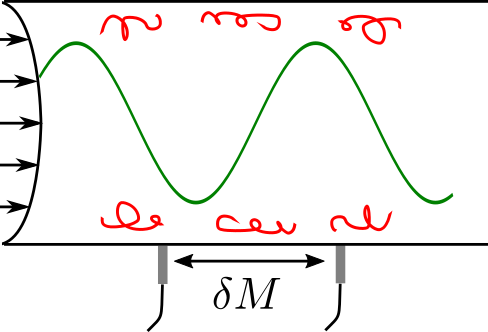
\includegraphics[width=3cm]{img/bruit.png}};
	\end{tikzpicture}
	%}\end{picture}
	}

\end{frame}



%%% CSM properties
%======================
%\section{CSM properties}
\begin{frame}[t]{Problem Statement}
	\begin{overlayarea}{\textwidth}{1.5cm}
	\only<1>{
	$$\underbracket[0.5pt]{~\bm{p}~}_{\text{measured spectra}} =\underbracket[0.5pt]{~\textcolor{green}{\bm{a}}~}_{\text{source spectra}} + \underbracket[0.5pt]{~\textcolor{red}{\bm{n}}~}_{\text{Gaussian noise}} $$
	}
	\only<2->{
	$$\Big\langle \underbracket[0.5pt]{~\bm{p}~}_{\text{measured spectra}} =\underbracket[0.5pt]{~\textcolor{green}{\bm{a}}~}_{\text{source spectra}} + \underbracket[0.5pt]{~\textcolor{red}{\bm{n}}~}_{\text{Gaussian noise}}  \Big\rangle_{\text{\normalsize $ N_s$ snapshots}}$$
	}
	\end{overlayarea}
	
	\onslide<2->{\textbf{Cross-Spectral Matrix} (covariance of Fourier component):
	$$\bm{S}_{pp} = \frac{1}{N_s} \sum_i  \bm{p}_i\bm{p}_i^H$$
	
	
	\begin{itemize}
		\item Hermitian (conjugate symmetric)
		\item Positive semidefinite (nonnegative eigenvalues)
	\end{itemize}~\\
	}

	\onslide<3->{
	$$\underbracket[0.5pt]{~\bm{S}_{pp}~}_{\text{measured CSM}} =\underbracket[0.5pt]{ ~\textcolor{green}{\bm{S}_{aa}}~}_{\text{signal of interest}} +\underbracket[0.5pt]{~\textcolor{red}{\bm{S}_{nn}}~}_{\text{unwanted noise}} + \underbracket[0.5pt]{~\bm{S}_{an}+\bm{S}_{na}}_{\text{cross-terms}}$$
	
	\begin{itemize}	
		\item Rank of $\textcolor{green}{\bm{S}_{aa}}=$ number of equivalent uncorrelated sources
	\end{itemize}
	}
\end{frame}

\begin{frame}{\insertsectionhead~--~CSM properties}
	\begin{overlayarea}{\textwidth}{3cm}

		\only<1>{$$\underbracket[0.5pt]{~\bm{S}_{pp}~}_{\text{measured CSM}} =\underbracket[0.5pt]{ ~\textcolor{green}{\bm{S}_{aa}}~}_{\text{signal of interest}} +\underbracket[0.5pt]{~\textcolor{red}{\bm{S}_{nn}}~}_{\parbox[t]{2cm}{\centering \text{\scriptsize unwanted noise}}} + \underbracket[0.5pt]{~\bm{S}_{an}+\bm{S}_{na}}_{\parbox[t]{2cm}{\centering \text{\scriptsize cross-terms}}}$$
		}
		
		\only<2>{$$\underbracket[0.5pt]{~\bm{S}_{pp}~}_{\text{measured CSM}} =\underbracket[0.5pt]{ ~\textcolor{green}{\bm{S}_{aa}}~}_{\text{signal of interest}} +\underbracket[0.5pt]{\bcancel{~\textcolor{red}{\bm{S}_{nn}}~}}_{\parbox[t]{2cm}{\centering \text{\scriptsize unwanted noise} \\ $\approx \diag{\textcolor{red}{\bm{\sigma}_n^2}}$ }} + \underbracket[0.5pt]{~\bm{S}_{an}+\bm{S}_{na}}_{\parbox[t]{2cm}{\centering \text{\scriptsize cross-terms}}}$$
		}
	
		\only<3>{$$\underbracket[0.5pt]{~\bm{S}_{pp}~}_{\text{measured CSM}} =\underbracket[0.5pt]{ ~\textcolor{green}{\bm{S}_{aa}}~}_{\text{signal of interest}} +\underbracket[0.5pt]{\bcancel{~\textcolor{red}{\bm{S}_{nn}}~}}_{\parbox[t]{2cm}{\centering \text{\scriptsize unwanted noise} \\ $\approx \diag{\textcolor{red}{\bm{\sigma}_n^2}}$ }} + \underbracket[0.5pt]{\bcancel{~\bm{S}_{an}+\bm{S}_{na}}}_{\parbox[t]{2cm}{\centering  \text{\scriptsize cross-terms}\\ $\rightarrow 0$ }}$$
		}
	
	\end{overlayarea}
	
	\hspace{0.8cm}\textbf{For $N_s \rightarrow \infty$}\\[1em]
	\pause
	\begin{itemize}
		\setlength{\itemindent}{1cm}
		\item Short correlation length : off-diagonal elements of $\textcolor{red}{\bm{S}_{nn}}\rightarrow 0$\\[1em]
		\pause
		\item Independent signal/noise : cross-terms $\rightarrow 0$
	\end{itemize}
	%$$\bm{S}_{pp} \approx \textcolor{green}{\bm{S}_{aa}} + \diag	{\textcolor{red}{\sigma^2}}$$

\end{frame}

%%% Plan
%======================
\begin{frame}{How to separate signal from noise ?}
	 
	
	\begin{itemize}
	%\setlength{\itemindent}{0.5cm}
		\item Existing methods:
			\begin{itemize}
			        \item 	3 diagonal reconstruction methods
		        		\item Robust Principal Component Analysis (RPCA)
			\end{itemize}
			
		\vfill\pause
	
		\item Proposed method: Probabilistic Factor Analysis

		\vfill \pause
		\item What is the influence on denoising performance of : 
		\begin{itemize}
		        \item noise level,
		        \item number of snapshots,
		        \item number of sources ?
		\end{itemize}
	\end{itemize}
\end{frame}


%%% Diagonal reconstruction
%======================
\section{Diagonal Reconstruction}
\begin{frame}
\tableofcontents[hideallsubsections]
\end{frame}
\begin{frame}
\tableofcontents[currentsection,hideothersubsections]
\end{frame}


\begin{frame}{\insertsectionhead}	
\hspace{-0.6cm}\textit{\small ``Remove as much noise as possible as long as denoised CSM remains non-negative''}
	\begin{block}{\normalsize Convex optimization   \citeTransp{Hald2017}}<2->
		\begin{equation*}
        			\text{maximize~} \| \textcolor{red}{\bm{\sigma}_{n}^2}\|_1 \text{~~subject to~~} \bm{S}_{pp}- \diag{\textcolor{red}{\bm{\sigma}_n^2}} \geq 0
		\end{equation*}
		{\small Problem solved with CVX Matlab toolbox}
	\end{block}
	\begin{block}{\normalsize Linear optimization \citeTransp{dougherty2016}}<3->
		\vspace{-0.2cm}
		\begin{equation*}
			\text{maximize~} \| \textcolor{red}{\bm{\sigma}_{n}^2}\|_1   \text{~~subject to~~}  \bm{V}^{H}_{(k-1)} \left( \bm{S}_{pp}- \diag{\textcolor{red}{\bm{\sigma}_n^2}}_{(k)} \right) \bm{V}_{(k-1)} \geq 0 
		\end{equation*}
		 $\bm{V}_{(k-1)}$: eigenvectors of $\bm{S}_{pp}-\diag{\textcolor{red}{\bm{\sigma}_n^2}}_{(1,...,k-1)} $\\[1pt]
		{\small Solved with \textit{linprog} Matlab function}
	\end{block}
	\begin{block}{\normalsize Alternating Projections  \citeTransp{leclere:hal-01279944}}<4->
		\begin{equation*}
        			 \bm{S}_{{pp}_{(k+1)}} := \bar{\bm{S}}_{{pp}_{(0)}} + \diag{\bm{V}^{H}_{(k)} \bm{s}_{(k)}^{\textcolor{orange}{\textbf{+}}}\bm{V}^{~}_{(k)}}
		\end{equation*}
		$\bm{V}_{(k)}$ and $\bm{s}_{(k)}$: eigenvectors/values of  $\bm{S}_{{pp}_{(k)}}$\\[1pt]
	\end{block}	
\end{frame}

%%% Test case
\subsection{Comparison on a test case}
\begin{frame}{\insertsectionhead~--~Test case}
	
	\begin{itemize}
	\item Default parameters:
		\noindent\begin{minipage}{1.1\linewidth}
		     	\begin{minipage}{0.4\linewidth}		     		
	         			\begin{itemize}
					\item 20  uncorrelated free field monopoles: \textcolor{red}{$\vcenter{\hbox{\tiny$\blacklozenge$}}$}
					\item 93 receivers: \textcolor{colorAlice}{$\vcenter{\hbox{\small$\bm{\circ}$}}$}
					\item SNR: 10 dB
					\item $10^4$ snapshots
					\item frequency: 15 kHz
				\end{itemize}	
	               		\vfill
	     		\end{minipage}
	      		%\hspace{0.02\linewidth}
	      		\hspace{0.5cm}
	     		 \begin{minipage}{0.5\linewidth}
             			\centering
             			\vspace{-0.5cm}
				% This file was created by matlab2tikz.
%
%The latest updates can be retrieved from
%  http://www.mathworks.com/matlabcentral/fileexchange/22022-matlab2tikz-matlab2tikz
%where you can also make suggestions and rate matlab2tikz.
%
\begin{tikzpicture}

\begin{axis}[%
width=4.3cm,
height=3cm,
at={(0cm,0cm)},
scale only axis,
xmin=-1,
xmax=1,
tick align=outside,
xlabel style={at={(0.15,0)}, font=\color{white!15!black},font=\scriptsize},
xlabel={x (m)},
ymin=-1,
ymax=0,
ylabel style={at={(0.7,-0.05)}, font=\color{white!15!black},font=\scriptsize},
ylabel={y (m)},
zmin=-1,
zmax=1,
zlabel style={at={(-0.08,0.5)}, font=\color{white!15!black},font=\scriptsize},
zlabel={z (m)},
view={-125.1}{10},
axis background/.style={fill=white},
axis x line*=bottom,
axis y line*=left,
axis z line*=left,
ytick={0,-0.5,-1},
xmajorgrids,
ymajorgrids,
zmajorgrids,
legend style={at={(0.2,1)}, anchor=south west, legend cell align=left, align=left, draw=white!15!black},
ticklabel style={font=\scriptsize}
]
\addplot3 [color=white, line width=1.0pt, draw=none, mark size=1.2pt, mark=o, mark options={line width=0.8pt,solid, colorAlice}]
 table[row sep=crcr] {%
0	-1	0\\
0.106660701334476	-1	0\\
0.0533000007271767	-1	0.092399999499321\\
-0.0533000007271767	-1	0.092399999499321\\
-0.106660701334476	-1	-9.31999988296184e-09\\
-0.0533000007271767	-1	-0.092399999499321\\
0.0533000007271767	-1	-0.092399999499321\\
0.196912005543709	-1	0\\
0.174356892704964	-1	0.091499999165535\\
0.111858800053596	-1	0.162055402994156\\
0.023700000718236	-1	0.195476293563843\\
-0.0697999969124794	-1	0.184115901589394\\
-0.147390797734261	-1	0.130576804280281\\
-0.191190093755722	-1	0.0471000000834465\\
-0.191190093755722	-1	-0.0471000000834465\\
-0.147390693426132	-1	-0.130576804280281\\
-0.0697999969124794	-1	-0.184115901589394\\
0.023700000718236	-1	-0.195476293563843\\
0.111858800053596	-1	-0.162055402994156\\
0.174356997013092	-1	-0.091499999165535\\
0.315122187137604	-1	0\\
0.287878394126892	-1	0.128171801567078\\
0.210857897996902	-1	0.23418140411377\\
0.09740000218153	-1	0.299699008464813\\
-0.0329000018537045	-1	0.313395887613297\\
-0.15756119787693	-1	0.272903800010681\\
-0.254939287900925	-1	0.18522410094738\\
-0.308236002922058	-1	0.0654999986290932\\
-0.308236002922058	-1	-0.0654999986290932\\
-0.25493910908699	-1	-0.185224294662476\\
-0.157560899853706	-1	-0.272903889417648\\
-0.0329000018537045	-1	-0.313395887613297\\
0.09740000218153	-1	-0.299698889255524\\
0.210858106613159	-1	-0.234181299805641\\
0.287878513336182	-1	-0.128171503543854\\
0.463685810565948	-1	0\\
0.432374089956284	-1	0.167502596974373\\
0.342667907476425	-1	0.312383085489273\\
0.206682503223419	-1	0.415074497461319\\
0.0428000018000603	-1	0.461707711219788\\
-0.126893594861031	-1	0.445984899997711\\
-0.279433101415634	-1	0.370029211044312\\
-0.394233614206314	-1	0.244099095463753\\
-0.455790609121323	-1	0.0851999968290329\\
-0.455790609121323	-1	-0.0851999968290329\\
-0.394233614206314	-1	-0.244099095463753\\
-0.279433101415634	-1	-0.370029211044312\\
-0.126893594861031	-1	-0.445984899997711\\
0.0428000018000603	-1	-0.461707800626755\\
0.206682503223419	-1	-0.415074497461319\\
0.342667788267136	-1	-0.312383085489273\\
0.432374089956284	-1	-0.167502596974373\\
0.672533094882965	-1	0\\
0.636093378067017	-1	0.218371197581291\\
0.530723094940186	-1	0.413078397512436\\
0.367840707302094	-1	0.563022196292877\\
0.165096998214722	-1	0.651953816413879\\
-0.0555000007152557	-1	0.670236110687256\\
-0.270153611898422	-1	0.615887820720673\\
-0.455494403839111	-1	0.494798600673676\\
-0.591475307941437	-1	0.32009020447731\\
-0.663360714912415	-1	0.110695198178291\\
-0.663360595703125	-1	-0.110695503652096\\
-0.591475129127502	-1	-0.320090502500534\\
-0.455494105815887	-1	-0.494798898696899\\
-0.270153313875198	-1	-0.615887880325317\\
-0.0555000007152557	-1	-0.670236110687256\\
0.165097206830978	-1	-0.651953816413879\\
0.367841005325317	-1	-0.563022017478943\\
0.530723392963409	-1	-0.413078010082245\\
0.636093497276306	-1	-0.218370899558067\\
0.899999976158142	-1	0\\
0.863543689250946	-1	0.253559291362762\\
0.757128119468689	-1	0.486576706171036\\
0.589374601840973	-1	0.680174589157104\\
0.3738734126091	-1	0.818668782711029\\
0.128083303570747	-1	0.890839278697968\\
-0.128083497285843	-1	0.890839278697968\\
-0.373873591423035	-1	0.818668723106384\\
-0.589374780654907	-1	0.68017452955246\\
-0.757128179073334	-1	0.486576706171036\\
-0.863543689250946	-1	0.253559112548828\\
-0.899999976158142	-1	-2.92999999373933e-07\\
-0.863543629646301	-1	-0.253559499979019\\
-0.757128119468689	-1	-0.486576914787292\\
-0.589374482631683	-1	-0.680174827575684\\
-0.373873203992844	-1	-0.818668901920319\\
-0.128083094954491	-1	-0.890839278697968\\
0.128083497285843	-1	-0.890839278697968\\
0.373873591423035	-1	-0.818668723106384\\
0.589375019073486	-1	-0.68017441034317\\
0.757128417491913	-1	-0.486576408147812\\
0.863543689250946	-1	-0.253559112548828\\
};
% \addlegendentry{Receivers}

\addplot3 [color=white, line width=1.0pt, draw=none, mark size=1.2pt, mark=diamond*, mark options={solid, fill=red, red}]
 table[row sep=crcr] {%
0.179001071858587	0	-1.19981625468941\\
0.181211485347157	0	-1.07351980682736\\
0.183421898835727	0	-0.94722335896532\\
0.185632312324296	0	-0.820926911103277\\
0.187842725812866	0	-0.694630463241235\\
0.190053139301436	0	-0.568334015379192\\
0.192263552790006	0	-0.442037567517149\\
0.194473966278576	0	-0.315741119655107\\
0.196684379767145	0	-0.189444671793064\\
0.198894793255715	0	-0.0631482239310213\\
0.201105206744285	0	0.0631482239310213\\
0.203315620232855	0	0.189444671793064\\
0.205526033721424	0	0.315741119655107\\
0.207736447209994	0	0.442037567517149\\
0.209946860698564	0	0.568334015379192\\
0.212157274187134	0	0.694630463241235\\
0.214367687675704	0	0.820926911103277\\
0.216578101164273	0	0.94722335896532\\
0.218788514652843	0	1.07351980682736\\
0.220998928141413	0	1.19981625468941\\
};
% \addlegendentry{Monopoles}

\end{axis}
\end{tikzpicture}%\\
				{\scriptsize \textcolor{black!50}{\hspace{0.5cm} From a benchmark case provided by PSA3}\vspace{-1cm}
}
	      		\end{minipage}
		\end{minipage}
	
	\item Varying parameters: \\
	\begin{itemize}
	        \item number of   \textcolor{red}{$\vcenter{\hbox{\tiny$\blacklozenge$}}$} (rank of $\textcolor{green}{\bm{S}_{aa}}$)\\[3pt]
	        \item SNR\\[3pt]
	        \item number of snapshots (level of extra-diagonal terms)
\end{itemize}~\\	
	
	\item Error on the signal CSM:
	\begin{equation*}
   		 \varepsilon = \frac{\|\diag{\textcolor{green}{\bm{S}_{aa}}}  - \diag{\textcolor{green}{\bm{\hat{S}}_{aa}}}\|_2}{\|\diag{\textcolor{green}{\bm{S}_{aa} }} \|_2}
	\end{equation*}
	\end{itemize}

\end{frame}


\begin{frame}{\insertsectionhead}

	%default values
	\small
	Default values:\\[1ex]
    \setlength\extrarowheight{3pt}
	\begin{tabular}{|c|c|c|c|c|}
	\hline
	 20  sources & 93 receivers & SNR: 10 dB & $10^4$ snapshots & frequency: 15 kHz	\\ \hline
	\end{tabular}
	
	\vfill


	%legend
%	\begin{mdframed}[
%		linecolor=black,%
%		innertopmargin =0.2cm,
%		innerbottommargin =0.2cm,
%		innerrightmargin =0.1cm,
%		innerleftmargin =0.1cm,
%		roundcorner=1pt
%		%usetwoside=true,
%		]		
		\definecolor{mycolor1}{rgb}{0.00000,0.44700,0.74100}%
		\definecolor{mycolor2}{rgb}{0.92900,0.69400,0.12500}%
		\definecolor{mycolor3}{rgb}{0.46600,0.67400,0.18800}%
		{\footnotesize \tikz[baseline=-1pt]\draw[line width=1.0pt,color=mycolor1](0,.5ex)--++(.5,0) ; Convex optimization \hfill
		\tikz[baseline=-1pt]\draw[color=mycolor2,line width=1.0pt] (0,.5ex)--++(.5,0) ; Alternating~projections\hfill
		 \tikz[baseline=-1pt]\draw[color=mycolor3,line width=1.0pt] (0,.5ex)--++(.5,0) ; Linear~optimization}
%	\end{mdframed}
	
	\resizebox{1.05\textwidth}{!}{
	\begin{minipage}{1.2\textwidth}
		\centering
		\hspace{-1cm}% This file was created by matlab2tikz.
%
%The latest updates can be retrieved from
%  http://www.mathworks.com/matlabcentral/fileexchange/22022-matlab2tikz-matlab2tikz
%where you can also make suggestions and rate matlab2tikz.
%
\definecolor{mycolor1}{rgb}{0.00000,0.44700,0.74100}%
\definecolor{mycolor2}{rgb}{0.92900,0.69400,0.12500}%
\definecolor{mycolor3}{rgb}{0.46600,0.67400,0.18800}%
%
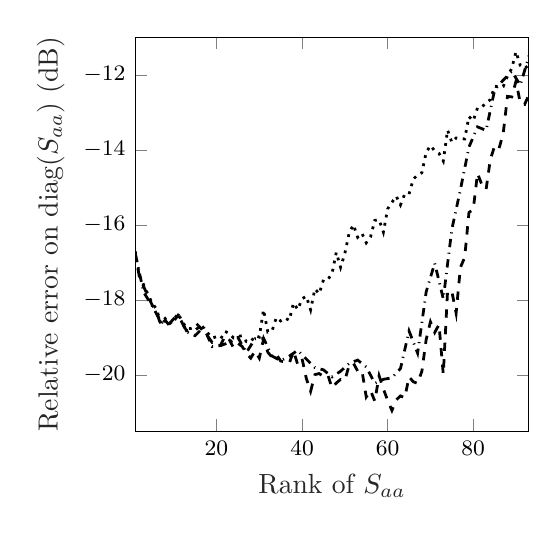
\begin{tikzpicture}

\begin{axis}[%
width=5cm,
height=5cm,
at={(0.698in,0.577in)},
scale only axis,
xmin=1,
xmax=93,
xlabel style={font=\color{white!15!black}},
xlabel={Rank of $\bo{S}_{aa}$},
ymin=-21.5,
ymax=-11,
ylabel style={font=\color{white!15!black}},
ylabel={Relative error on diag($\bo{S}_{aa}$) (dB)},
axis background/.style={fill=white},
%legend style={at={(0.03,0.97)}, anchor=north west, legend cell align=left, align=left, draw=white!15!black},
ticklabel style={font=\footnotesize}
]
\addplot [dashed, line width=1.0pt]
  table[row sep=crcr]{%
1	-16.7370680069206\\
2	-17.4012486274349\\
3	-17.6491818488274\\
4	-17.9064077264361\\
5	-18.1447068295614\\
6	-18.2991015940721\\
7	-18.6889443982282\\
8	-18.5431609994158\\
9	-18.6827904229415\\
10	-18.5674269671433\\
11	-18.4151877420299\\
12	-18.6155581391726\\
13	-18.8241402547782\\
14	-18.7968579237859\\
15	-18.8115559647255\\
16	-18.7177312875175\\
17	-18.8426847100225\\
18	-18.9769685037876\\
19	-19.1386182787638\\
20	-19.1008264439063\\
21	-19.2019012624285\\
22	-18.9638333040042\\
23	-19.064854318432\\
24	-19.2814348480029\\
25	-19.1579739293932\\
26	-19.242148720853\\
27	-19.4294848873866\\
28	-19.5544470906725\\
29	-19.3642942895123\\
30	-19.5553874354648\\
31	-19.0500959146534\\
32	-19.3987697900783\\
33	-19.5304514228384\\
34	-19.4542712225361\\
35	-19.6325505796662\\
36	-19.6557273851441\\
37	-19.7002414716667\\
38	-19.3629820152635\\
39	-19.7284199656174\\
40	-19.5725136563716\\
41	-20.0969027170615\\
42	-20.4392752387639\\
43	-19.9942426610875\\
44	-19.9660307154902\\
45	-20.0429018825232\\
46	-19.9979893621137\\
47	-20.3468095355529\\
48	-20.2173084142236\\
49	-20.1220446519779\\
50	-20.1488771858363\\
51	-19.7417251549062\\
52	-19.6902325698739\\
53	-19.9006921955836\\
54	-19.8879044378504\\
55	-20.5906777578333\\
56	-20.4214753811965\\
57	-20.6993699221106\\
58	-20.0249204995815\\
59	-20.3744029357285\\
60	-20.6821067503624\\
61	-20.9493207523177\\
62	-20.6687842833634\\
63	-20.5624430140821\\
64	-20.610588300034\\
65	-20.0530916504033\\
66	-20.185354157788\\
67	-20.2276578199841\\
68	-19.9032895993565\\
69	-19.0588890939865\\
70	-18.5863609062983\\
71	-18.8694241807615\\
72	-18.6615080569044\\
73	-19.9855563428767\\
74	-17.7650637298136\\
75	-17.7742442988787\\
76	-18.3525056361618\\
77	-17.1355757602416\\
78	-16.8680058512031\\
79	-15.6690487660575\\
80	-15.5924789735929\\
81	-14.6253911519703\\
82	-14.9255677835853\\
83	-15.0592102025514\\
84	-14.2479761559614\\
85	-13.9011811248436\\
86	-13.9749878665702\\
87	-13.5648292386533\\
88	-12.5738968125401\\
89	-12.5872476645548\\
90	-12.1658621412658\\
91	-12.7574703314859\\
92	-12.7892285383686\\
93	-12.5352552536202\\
};
%\addlegendentry{Hald}

\addplot [dotted, line width=1.0pt]
  table[row sep=crcr]{%
1	-16.7031735568394\\
2	-17.3615793178814\\
3	-17.6023910194524\\
4	-17.8590648144034\\
5	-18.0920512541652\\
6	-18.2471658246905\\
7	-18.6317902239427\\
8	-18.4977628924507\\
9	-18.6416131210868\\
10	-18.5407206938205\\
11	-18.3579547122712\\
12	-18.5777123716674\\
13	-18.7558275781406\\
14	-18.7638375252025\\
15	-18.7263046755914\\
16	-18.6171722924591\\
17	-18.7484458200624\\
18	-18.8889996301139\\
19	-19.0168545785086\\
20	-18.9838969852324\\
21	-19.0362411600279\\
22	-18.839047714971\\
23	-18.8992114751233\\
24	-19.0178392942204\\
25	-18.973372504287\\
26	-18.9570601283013\\
27	-19.1151606755411\\
28	-19.1243272889151\\
29	-18.9565947336197\\
30	-18.9928166456091\\
31	-18.2607754921369\\
32	-18.8577390142871\\
33	-18.8207458681384\\
34	-18.4703448119709\\
35	-18.5628723202705\\
36	-18.482213292984\\
37	-18.5467169963642\\
38	-18.084578041105\\
39	-18.2584746338685\\
40	-17.971037041929\\
41	-17.903047167223\\
42	-18.2656334735752\\
43	-17.7076249942603\\
44	-17.8376474130466\\
45	-17.466483854883\\
46	-17.4619805785055\\
47	-17.2992973591824\\
48	-16.7349922629297\\
49	-17.1332353760362\\
50	-16.7608127883464\\
51	-16.2208561368426\\
52	-15.9977348834246\\
53	-16.3301175422647\\
54	-16.2236308580102\\
55	-16.4790123468826\\
56	-16.321755676887\\
57	-15.879582444345\\
58	-15.8646249867458\\
59	-16.1948135221325\\
60	-15.5748336292661\\
61	-15.3997315246477\\
62	-15.234409444078\\
63	-15.4677813038868\\
64	-15.1770932535575\\
65	-15.1816264878348\\
66	-14.7782694354678\\
67	-14.672705322969\\
68	-14.6103285259422\\
69	-14.0679838246761\\
70	-13.8842756145066\\
71	-14.0280701886142\\
72	-14.0938964953599\\
73	-14.2992026516806\\
74	-13.4728675177465\\
75	-13.798481796497\\
76	-13.6827485542733\\
77	-13.6989927630093\\
78	-13.7094398967119\\
79	-13.1123448054893\\
80	-13.224050392688\\
81	-12.8794359933912\\
82	-12.8656537446746\\
83	-12.737455902532\\
84	-12.6632329496487\\
85	-12.302605699363\\
86	-12.3235831340387\\
87	-12.31224796278\\
88	-12.0359657066058\\
89	-11.8260147055477\\
90	-11.3800766460464\\
91	-11.7510755848985\\
92	-11.8312307358659\\
93	-11.7345525555786\\
};
%\addlegendentry{Basic AP}

\addplot [dashdotted, line width=1.0pt]
  table[row sep=crcr]{%
1	-16.7703982586393\\
3	-17.8027151264291\\
5	-18.1611873996741\\
7	-18.5900852562987\\
9	-18.632952980168\\
11	-18.3799571387113\\
13	-18.8526332108527\\
15	-18.9544741723528\\
17	-18.7292293213212\\
19	-19.2469736370832\\
21	-19.2178482051645\\
23	-19.1364318772276\\
25	-19.002911767836\\
27	-19.4050146207132\\
29	-19.0363195257525\\
31	-19.0255108139849\\
33	-19.4993485181015\\
35	-19.6244673423558\\
37	-19.5010227306989\\
39	-19.3437531422468\\
41	-19.5812435179046\\
43	-19.8064889271868\\
45	-19.8669692137437\\
47	-20.0535199803389\\
49	-19.9043121154516\\
51	-19.6953212351942\\
53	-19.6063060044982\\
55	-19.7898785505215\\
57	-20.2254647962434\\
59	-20.1194587509014\\
61	-20.0802403259681\\
63	-19.8313662116886\\
65	-18.8303511930449\\
67	-19.421731301575\\
69	-17.787171194203\\
71	-17.0220868605511\\
73	-17.9734205941633\\
75	-16.116977060264\\
77	-15.0632511061207\\
79	-13.9259539749941\\
81	-13.3870312552658\\
83	-13.4807282912676\\
85	-12.4027224224411\\
87	-12.1404124603201\\
89	-11.906610936308\\
91	-12.2742304982996\\
93	-11.5016690329509\\
95	-11.2624167819261\\
};
%\addlegendentry{Dougherty}

\end{axis}
\end{tikzpicture}%
		\hspace{-0.2cm}% This file was created by matlab2tikz.
%
%The latest updates can be retrieved from
%  http://www.mathworks.com/matlabcentral/fileexchange/22022-matlab2tikz-matlab2tikz
%where you can also make suggestions and rate matlab2tikz.
%
\definecolor{mycolor1}{rgb}{0.00000,0.44700,0.74100}%
\definecolor{mycolor2}{rgb}{0.92900,0.69400,0.12500}%
\definecolor{mycolor3}{rgb}{0.46600,0.67400,0.18800}%
%
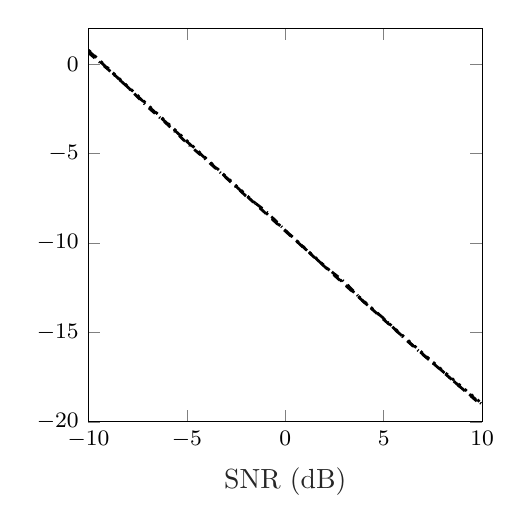
\begin{tikzpicture}

\begin{axis}[%
width=5cm,
height=5cm,
at={(0.698in,0.577in)},
scale only axis,
xmin=-10,
xmax=10,
xlabel style={font=\color{white!15!black}},
xlabel={SNR (dB)},
ymin=-20,
ymax=2,
ylabel style={font=\color{white!15!black}},
%ylabel={Relative error on diag($\bo{S}_{aa}$) (dB)},
axis background/.style={fill=white},
%legend style={legend cell align=left, align=left, draw=white!15!black,draw=none},
ticklabel style={font=\footnotesize}
]
\addplot [dashed, line width=1.0pt]
  table[row sep=crcr]{%
-10	0.741936726042635\\
-9	-0.279871558906809\\
-8	-1.29793889872774\\
-7	-2.31250215060388\\
-6	-3.32385843940163\\
-5	-4.33231602157427\\
-4	-5.33815606764263\\
-3	-6.34160607693496\\
-2	-7.34282285173506\\
-1	-8.34188162702269\\
0	-9.33876820590928\\
1	-10.3333716946942\\
2	-11.3254761499002\\
3	-12.3147500446174\\
4	-13.3007328082572\\
5	-14.2828183557954\\
6	-15.2602355911512\\
7	-16.2320269339108\\
8	-17.1970261939449\\
9	-18.1538385636966\\
10	-19.1008264439063\\
};
%\addlegendentry{Hald}

\addplot [dotted, line width=1.0pt]
  table[row sep=crcr]{%
-10	0.779421806215343\\
-9	-0.24126724351376\\
-8	-1.2587825204969\\
-7	-2.27316989167413\\
-6	-3.28457344364643\\
-5	-4.29316850330374\\
-4	-5.29920728111668\\
-3	-6.30284069033434\\
-2	-7.30418337336454\\
-1	-8.30320818198451\\
0	-9.29993911720495\\
1	-10.2942467561698\\
2	-11.2858442520237\\
3	-12.2743259057356\\
4	-13.2591427383762\\
5	-14.2393693711815\\
6	-15.2136600616136\\
7	-16.1798762054949\\
8	-17.1349033154619\\
9	-18.0728513427519\\
10	-18.9838969852324\\
};
%\addlegendentry{Basic AP}

\addplot [dashdotted, line width=1.0pt]
  table[row sep=crcr]{%
-10	0.632409149389929\\
-9	-0.303634924009498\\
-8	-1.29980052352317\\
-7	-2.39207793841264\\
-6	-3.36666184772421\\
-5	-4.41843225036159\\
-4	-5.37652523103519\\
-3	-6.36645613251494\\
-2	-7.37776074985382\\
-1	-8.21329471199083\\
0	-9.29424456455585\\
1	-10.3202840883304\\
2	-11.3115681168112\\
3	-12.161287691351\\
4	-13.3139607304893\\
5	-14.2143644335812\\
6	-15.2928155848239\\
7	-16.2517519665826\\
8	-17.1780406048299\\
9	-18.1601577959815\\
10	-19.0187185721311\\
};
%\addlegendentry{Dougherty}

\end{axis}
\end{tikzpicture}%
		\hspace{-0.4cm}% This file was created by matlab2tikz.
%
%The latest updates can be retrieved from
%  http://www.mathworks.com/matlabcentral/fileexchange/22022-matlab2tikz-matlab2tikz
%where you can also make suggestions and rate matlab2tikz.
%
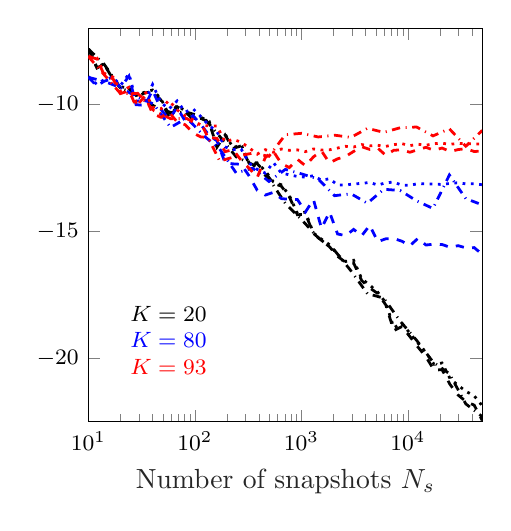
\begin{tikzpicture}

\begin{axis}[%
width=5cm,
height=5cm,
at={(0.698in,0.577in)},
scale only axis,
xmode=log,
xmin=10,
xmax=50000,
xminorticks=true,
xlabel style={font=\color{white!15!black}},
xlabel={Number of snapshots $N_s$},
ymin=-22.5,
ymax=-7,
ylabel style={font=\color{white!15!black}},
%ylabel={Relative error on diag($\bm{S}_{aa}$) (dB)},
axis background/.style={fill=white},
%legend style={at={(0.03,0.03)}, anchor=south west, legend cell align=left, align=left, fill=none, draw=none},
ticklabel style={font=\footnotesize}
]
\addplot [color=black, dashed, line width=1.0pt]
  table[row sep=crcr]{%
10	-7.82333428697925\\
12	-8.56825865789703\\
14	-8.41307189268658\\
17	-9.00920407597321\\
20	-9.3537297457783\\
24	-9.38154480575806\\
28	-9.69933077355055\\
34	-9.54572626890163\\
40	-9.49363876448267\\
48	-9.83152364928392\\
57	-10.4989520844455\\
68	-10.0885165297253\\
81	-10.289242068753\\
96	-10.5910772256717\\
114	-10.551256659757\\
136	-10.6999195584293\\
161	-11.6822360514168\\
192	-11.2036718289485\\
228	-11.7326383786081\\
272	-11.6321736070583\\
323	-12.3461673158785\\
385	-12.3335241899759\\
458	-12.6797802976475\\
545	-13.1071311573618\\
648	-13.218232503601\\
771	-13.638765374058\\
918	-14.3451312802867\\
1092	-14.3163721616522\\
1299	-15.0794082432676\\
1546	-15.3479160018766\\
1839	-15.6058416506055\\
2189	-15.9796665756589\\
2604	-16.2181576360932\\
3098	-16.2453137480635\\
3687	-16.9325089051901\\
4387	-17.2237873292114\\
5219	-17.445299955056\\
6210	-17.8927718684032\\
7389	-18.9052275179887\\
8792	-18.7444702910516\\
10461	-19.1412845745748\\
12447	-19.5517487895886\\
14810	-19.9365780357358\\
17621	-20.4592505267682\\
20966	-20.4442853610926\\
24947	-21.0280333556023\\
29683	-21.4419733827312\\
35318	-21.7022069388402\\
42022	-21.839653350729\\
50000	-22.4400803719689\\
};
%\addlegendentry{Hald}

\addplot [color=black, dotted, line width=1.0pt]
  table[row sep=crcr]{%
10	-7.80793444781493\\
12	-8.54357234510443\\
14	-8.39469514057678\\
17	-8.98371296425242\\
20	-9.3101201341527\\
24	-9.34059800029062\\
28	-9.64825236997246\\
34	-9.51225679351986\\
40	-9.43386375730012\\
48	-9.77951121147543\\
57	-10.4193291725435\\
68	-10.0379120952645\\
81	-10.2573112531791\\
96	-10.5586968410626\\
114	-10.5084519556703\\
136	-10.6607374022787\\
161	-11.6366904050299\\
192	-11.1646612483853\\
228	-11.7090090135855\\
272	-11.5828455868267\\
323	-12.3119340391412\\
385	-12.2961968775694\\
458	-12.6139941963631\\
545	-13.0462003552294\\
648	-13.164294408213\\
771	-13.5852880495537\\
918	-14.2886191897588\\
1092	-14.240923911883\\
1299	-15.0626456778487\\
1546	-15.3070545686674\\
1839	-15.5220368679069\\
2189	-15.9174132191443\\
2604	-16.1826401774589\\
3098	-16.1347602952486\\
3687	-16.8636455530214\\
4387	-17.1103588814124\\
5219	-17.3923233267944\\
6210	-17.808185727603\\
7389	-18.7954459777261\\
8792	-18.6127800084382\\
10461	-19.0080069318031\\
12447	-19.3990249536675\\
14810	-19.7751973105429\\
17621	-20.2296220421925\\
20966	-20.1802510326307\\
24947	-20.7961953526922\\
29683	-21.0595998378458\\
35318	-21.3013727638665\\
42022	-21.473265640537\\
50000	-21.8618900925979\\
};
%\addlegendentry{Basic AP}

\addplot [color=black, dashdotted, line width=1.0pt]
  table[row sep=crcr]{%
10	-7.82333428699501\\
14	-8.41307189274591\\
20	-9.35372974578693\\
29	-9.63226374349065\\
41	-10.056806638212\\
59	-10.3160387339534\\
84	-10.3049677497188\\
120	-10.5051609432566\\
171	-11.2595840432922\\
244	-12.0640998211784\\
348	-12.3633902035622\\
496	-12.9177426253893\\
707	-13.8970601211009\\
1008	-14.5430890893978\\
1438	-15.2498805656574\\
2050	-15.7474277967298\\
2924	-16.5527174272982\\
4170	-17.4486278403843\\
5946	-17.6268302116185\\
8479	-18.5343612923237\\
12091	-19.2863256678069\\
17242	-20.1388078820684\\
24588	-20.6028943537641\\
35063	-21.790971614331\\
50000	-22.2895980979102\\
};
%\addlegendentry{Dougherty}

\addplot [color=blue, dashed, line width=1.0pt, forget plot]
  table[row sep=crcr]{%
10	-8.93603352053439\\
12	-9.2768274080883\\
14	-9.08867791021664\\
17	-8.97293812761002\\
20	-9.33817825943744\\
24	-8.88462701625932\\
28	-10.0096200883148\\
34	-10.0400104005013\\
40	-9.43669891860869\\
48	-10.1952209505627\\
57	-10.5835922323244\\
68	-10.1224955259962\\
81	-10.6571028028582\\
96	-10.4446124095427\\
114	-10.7971816527864\\
136	-11.2269162979536\\
161	-11.4321954065187\\
192	-12.2994620620593\\
228	-12.3399862753503\\
272	-12.3582049927563\\
323	-12.8179243721615\\
385	-13.3801205009488\\
458	-13.5673131755681\\
545	-13.4623880609512\\
648	-13.706901141978\\
771	-13.7384766890607\\
918	-13.7439778657591\\
1092	-14.2314408456603\\
1299	-13.7482336014909\\
1546	-14.8772495623418\\
1839	-14.2378082368479\\
2189	-15.1004952527464\\
2604	-15.1643666809034\\
3098	-14.9205180459622\\
3687	-15.1710642548613\\
4387	-14.7597761010359\\
5219	-15.4037714546301\\
6210	-15.2900712707957\\
7389	-15.2779020230199\\
8792	-15.3839305195171\\
10461	-15.5630177447767\\
12447	-15.2736633780203\\
14810	-15.5361295278176\\
17621	-15.4995188975361\\
20966	-15.5141415136162\\
24947	-15.6253845993813\\
29683	-15.5608872243312\\
35318	-15.6504539560966\\
42022	-15.6373239622894\\
50000	-15.9007681103558\\
};
\addplot [color=blue, dotted, line width=1.0pt, forget plot]
  table[row sep=crcr]{%
10	-8.90475826584368\\
12	-9.21087904806858\\
14	-9.02736475364325\\
17	-8.92677824536293\\
20	-9.25263714755025\\
24	-8.79345973378303\\
28	-9.86608237845375\\
34	-9.85743927953508\\
40	-9.21356418507511\\
48	-9.93188404591018\\
57	-10.1795657287298\\
68	-9.86294298773716\\
81	-10.2985728695485\\
96	-10.1729271661589\\
114	-10.4862201864306\\
136	-10.8278326228668\\
161	-11.072923185335\\
192	-11.6739225365932\\
228	-11.7748217648389\\
272	-11.7577495657563\\
323	-12.3109956030518\\
385	-12.5565958708607\\
458	-12.7043097427035\\
545	-12.2834024472871\\
648	-12.7033553818168\\
771	-12.7704829688464\\
918	-12.8370147352328\\
1092	-12.8613429720553\\
1299	-12.8076041920794\\
1546	-12.9836006678977\\
1839	-12.9255094535016\\
2189	-13.1692601945706\\
2604	-13.1729550367025\\
3098	-13.1294460567847\\
3687	-13.1105664544967\\
4387	-13.0698225451343\\
5219	-13.1772775019131\\
6210	-13.0827893907747\\
7389	-13.0585351986582\\
8792	-13.1799571529658\\
10461	-13.1815881505353\\
12447	-13.1204458426834\\
14810	-13.1270657724956\\
17621	-13.1306049433544\\
20966	-13.1546282504014\\
24947	-13.1073341513408\\
29683	-13.0840290937792\\
35318	-13.1293756307948\\
42022	-13.122490352446\\
50000	-13.1619054581311\\
};
\addplot [color=blue, dashdotted, line width=1.0pt, forget plot]
  table[row sep=crcr]{%
10	-8.93603352054036\\
14	-9.08867791026314\\
20	-9.33817825946941\\
29	-9.72192574601124\\
41	-9.98499570703256\\
59	-10.9057428749612\\
84	-10.5351609126483\\
120	-11.2157406566542\\
171	-11.7562627861008\\
244	-12.699637435584\\
348	-12.5086536798054\\
496	-13.0338266385178\\
707	-12.5572769572184\\
1008	-12.7372909362437\\
1438	-12.9361089100873\\
2050	-13.5933918912477\\
2924	-13.5159417017122\\
4170	-13.8906103758171\\
5946	-13.3411758311276\\
8479	-13.3889369963427\\
12091	-13.7959592382385\\
17242	-14.0963452040554\\
24588	-12.7779837842823\\
35063	-13.7081230496966\\
50000	-13.9541640228626\\
};
\addplot [color=red, dashed, line width=1.0pt, forget plot]
  table[row sep=crcr]{%
10	-8.11999862056285\\
12	-8.20917879115695\\
14	-8.82446572200605\\
17	-8.99396139972689\\
20	-9.57314674595566\\
24	-9.46129905382258\\
28	-10.074934933022\\
34	-9.66691947618468\\
40	-10.3622598643397\\
48	-10.5074906891077\\
57	-10.3053415974817\\
68	-10.6882347785008\\
81	-10.7984884233697\\
96	-11.1222485168622\\
114	-11.2826331528717\\
136	-11.2990452618958\\
161	-11.3403305721596\\
192	-11.857844131995\\
228	-11.7811637738906\\
272	-12.2005746184346\\
323	-12.5106033556634\\
385	-12.8757827310285\\
458	-12.0884206403229\\
545	-11.843434396461\\
648	-12.3271489953751\\
771	-12.4839305520084\\
918	-12.159352539392\\
1092	-12.4160368110383\\
1299	-12.0645459302025\\
1546	-11.8330519428547\\
1839	-12.3027137985051\\
2189	-12.1423126490061\\
2604	-12.048455609738\\
3098	-11.8498346104671\\
3687	-11.6646016991927\\
4387	-11.7701672954647\\
5219	-11.720483731987\\
6210	-12.0057225151849\\
7389	-11.8029049969001\\
8792	-11.7920431969372\\
10461	-11.8825384213489\\
12447	-11.7801266416599\\
14810	-11.6895244986989\\
17621	-11.8064865100467\\
20966	-11.716349947916\\
24947	-11.8544083960463\\
29683	-11.7775456710281\\
35318	-11.7411595183262\\
42022	-11.8548454423014\\
50000	-11.832289239983\\
};
\addplot [color=red, dotted, line width=1.0pt, forget plot]
  table[row sep=crcr]{%
10	-8.10924276715784\\
12	-8.1688235797982\\
14	-8.77091396664955\\
17	-8.92360954989237\\
20	-9.48190339333175\\
24	-9.32422570677304\\
28	-9.90544763806884\\
34	-9.48322412081793\\
40	-10.1137358307318\\
48	-10.1739708540527\\
57	-9.84105596998775\\
68	-10.216392244428\\
81	-10.447524861844\\
96	-10.6075789395958\\
114	-10.8225219785817\\
136	-10.8446980164261\\
161	-10.8496527397411\\
192	-11.4812937886717\\
228	-11.3700782190028\\
272	-11.4898300101081\\
323	-11.7087345111466\\
385	-11.956185921804\\
458	-11.7819786023685\\
545	-11.8830215679093\\
648	-11.7558431960859\\
771	-11.8090715885033\\
918	-11.7897543588438\\
1092	-11.85846292126\\
1299	-11.7523872982692\\
1546	-11.7970879311299\\
1839	-11.7872312939611\\
2189	-11.7173332489399\\
2604	-11.6495781747231\\
3098	-11.6764245994724\\
3687	-11.5818087251356\\
4387	-11.6281651893558\\
5219	-11.6095425706171\\
6210	-11.6519783332185\\
7389	-11.5826153982752\\
8792	-11.5440825885452\\
10461	-11.623834389775\\
12447	-11.5660006831206\\
14810	-11.6072808958992\\
17621	-11.5454897169953\\
20966	-11.5301087339078\\
24947	-11.5682332932596\\
29683	-11.5376862728834\\
35318	-11.5451701107758\\
42022	-11.5544284049644\\
50000	-11.5556882514815\\
};
\addplot [color=red, dashdotted, line width=1.0pt, forget plot]
  table[row sep=crcr]{%
10	-8.11999862058022\\
14	-8.82446572202169\\
20	-9.57314674598619\\
29	-9.56500185963869\\
41	-10.2383851718711\\
59	-10.5614269565543\\
84	-10.5574668659871\\
120	-10.9245333549993\\
171	-12.2311464912163\\
244	-12.0419106789052\\
348	-11.9194142897316\\
496	-12.0410611829043\\
707	-11.1943998241216\\
1008	-11.1361299838029\\
1438	-11.2814989877562\\
2050	-11.210873822398\\
2924	-11.2982093042418\\
4170	-10.9402499670014\\
5946	-11.0996495249546\\
8479	-10.9184253586683\\
12091	-10.8895596066784\\
17242	-11.2379554382587\\
24588	-10.9605425250878\\
35063	-11.6455139049923\\
50000	-11.0237161014279\\
};

\node[anchor=south west, align=left,font= \footnotesize]
at (axis cs:20,-21) {$K=20$\\\textcolor{blue}{$K=80$}\\\textcolor{red}{$K=93$}};
\end{axis}
\end{tikzpicture}%
	\end{minipage}
	}
	\begin{block}{Select Convex Optimization (DRec) for further comparison}
		\ding{51} Fast, simple code		 \hfill\parbox{0.5\linewidth}{\ding{55} Local optimization}\\
		\ding{51} Better performance		 \hfill\parbox{0.5\linewidth}{\ding{55} Denoises only auto-spectra}\\
	\end{block}

\end{frame}

%%% RPCA
%======================
\section{Robust Principal Component Analysis}
\begin{frame}
\tableofcontents[currentsection,hideothersubsections]
\end{frame}
\begin{frame}{RPCA}
	\vspace{-0.5cm}
	\begin{center}
		\textit{``Search \textcolor{green}{$\bm{S}_{aa}$} as a low rank matrix and \textcolor{red}{$\bm{S}_{nn}$} as a sparse matrix''}\\~\\
		\colorbox{gray!20}{
		 $\text{minimize~} \|\textcolor{green}{\bm{{S}}_{aa}} \|_* + \lambda \| \textcolor{red}{\bm{{S}}_{nn}} \|_1  \text{~~~~subject to~~~~} \textcolor{green}{ \bm{{S}}_{aa}} +  \textcolor{red}{\bm{{S}}_{nn}} = \bm{S}_{pp}$
		}
	\end{center}


	
	$\| \cdot \|_*$: nuclear norm (sum of eigenvalues: related to rank)\\
	$\| \cdot \|_1$: $\ell_1$-norm (related to sparsity)\\~\\
	
	Solved with a proximal gradient algorithm
	\vfill

	\begin{block}{RPCA  \citeTransp{Wright2009a}}
		\ding{51} Modifies the whole CSM		\hfill\parbox{0.56\linewidth}{\ding{55} Local optimization}\\[2pt]
		\parbox{0.42\linewidth}{\ding{51} Widely used in image\\ processing}\hfill\parbox{0.56\linewidth}{\ding{55} Choose regularization parameter:
		\small
		\begin{itemize}
			\setlength{\itemindent}{0.3cm}
		        \item[-] L-curve criterion,\\[-2pt]
		        \item[-] Generalized cross validation method,\\[-2pt]
		       \item[-] Bayesian criterion, \dots
		\end{itemize}
		}
	\end{block}
	\vfill
	\begin{tabular}{rl}
	$\hookrightarrow$ For comparison :& - optimal $\lambda$  (unknown on real case)\\
	& - ``universal'' constant  parameter $\lambda=M^{-\frac{1}{2}}=0.1$
	\end{tabular}

\end{frame}

%%% PFA
%======================
\section{Probabilistic Factor Analysis}
\begin{frame}
\tableofcontents[currentsection,hideothersubsections]
\end{frame}

\begin{frame}{\insertsectionhead}
	\vspace{-0.5em}
	\begin{itemize}
        		\item<1-> \textbf{Latent variable model}\\    ~\\    		
        		\hspace{-2em}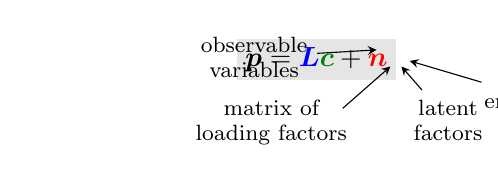
\begin{tikzpicture}[remember picture]
			\colorbox{gray!20}{$\tikzmark{p}\bm{p} = \tikzmark{L}\textcolor{blue}{\bm{L}} \tikzmark{c}\textcolor{green}{\bm{c}} + \tikzmark{n}\textcolor{red}{\bm{n}}$}
			
			%p
			\node (pdescr) [below left=-0.5cm and 1cm of p, align=center]{
				\footnotesize observable\\[-3pt] \footnotesize variables
			};
			\draw[->,>=stealth] (pdescr) -- ($(p.east)+(-7pt,6pt)$);
			
			% L
			\node(Ldescr) [below left=0.3cm and 0.5cm of L,align=center] {
				\footnotesize matrix of\\[-3pt] \footnotesize loading factors
			};
	    		%\draw[] (Ldescr.east) to [in=-90,out=45]  (L.south) ;
	    		\draw[->,>=stealth] ($(Ldescr.east)+(-5pt,5pt)$) to ($(L)+(-2pt,0)$);
	    		
	    		% c
	    		\node(cdescr) [below right  =0.3cm  and 0.1cm of c , align=center]{
	    			\footnotesize latent\\[-3pt] \footnotesize factors
	    		};
	    		\draw[->,>=stealth] (cdescr) to ($(c.south)+(2pt,0)$);
	    		
	    		% n
	    		\node(ndescr) [below right=0.2cm and 1cm of n,align=center]{
	    			\footnotesize error (noise)
	    		};
	    		\draw[->,>=stealth] (ndescr) to ($(n)+(5pt,2pt)$);
		\end{tikzpicture}
		
		\begin{itemize}
		        \item Capture dominant correlation with fewer parameters (close to PCA) 
		        \item Extract anisotropic noise\pause
		\end{itemize}
	\end{itemize}
        	\begin{overlayarea}{\textwidth}{0.5\textheight}
        	\only<2-4>{
	\begin{itemize}        		
        		\item \textbf{Statistical inference: }See parameters as random variables
        		\vspace{-0.2cm}\begin{multicols}{3}
		\hspace{0.5cm}$\textcolor{blue}{\bm{L}}\sim\mathcal{N}_{\mathbb{C}}(0,\bm{\gamma}^2)$\\
		\hspace{0.2cm}$\textcolor{green}{\bm{c}}\sim\mathcal{N}_{\mathbb{C}}(0,\bm{I\alpha}^2)$\\
		\hspace{0.2cm}$\textcolor{red}{\bm{n}}\sim\mathcal{N}_{\mathbb{C}}(0,\bm{I\sigma}^2)$\\
		\end{multicols}
		\vspace{-0.2cm}+ non-informative priors : $\bm{\gamma}^2, \bm{\alpha}^2, \bm{\sigma}^2\sim\mathcal{IG}(a_{\gamma,\alpha,\sigma},b_{\gamma,\alpha,\sigma})$\\[1ex]      	
		\pause			 
        		   \vfill     		
        		\item \textbf{Solved using MCMC algorithm} (Gibbs sampling)\\
		\small Iterative draws in the marginal conditional distributions of each parameter\normalsize
		\pause		
        		 \vfill 
        		 \vspace{-0.5em}
        		 \item \textbf{Finally}, signal CSM: 
        		 \hspace{4ex}\parbox{0.3\textwidth}{
        		 $$\bm{\hat{S}}_{aa}=\frac{1}{N_s}\sum_{i=1}^{N_s}\textcolor{blue}{\bm{L}}\textcolor{green}{\bm{c}}_i\textcolor{green}{\bm{c}}^H_i\textcolor{blue}{\bm{L}}^H$$        
        		}
		 
	\end{itemize}
	}	
	\only<5->{
	\begin{block}{PFA}
		\ding{51} Global optimization \hfill\parbox{0.5\linewidth}{\ding{55} Computationally expensive}\\
		\ding{51} Flexible model\\
		\ding{51} Cross-terms  taken into account in the model
	\end{block}~\\
	}
	\end{overlayarea}	
\end{frame}

%\begin{frame}{\insertsectionhead}
%	\begin{itemize}
%	        \item 	Gibbs sampling in the Bayesian hierarchical model : \\[.5cm]
%		\hspace{-1.7cm}\begin{tikzpicture}[remember picture]
%			$\bm{p} = \tikzmark{L}\bm{L}   \tikzmark{c}\bm{c} + \tikzmark{n}\bm{n}$
%			
%			% L
%			\node(Ldescr) [below left=0.5cm and 2cm of L,align=center] {
%				Loading factors\\
%				$\bm{L}\sim\mathcal{N}_{\mathbb{C}}(0,\bm{\gamma}^2)$
%			};
%	    		%\draw[] (Ldescr.east) to [in=-90,out=45]  (L.south) ;
%	    		\draw[] (Ldescr.east)++(0,10pt) to [in=-130,out=45] (L);
%	    		
%	    		% c
%	    		\node(cdescr) [below  =0.5cm  of c,align=center]{
%	    			Latent variables\\
%	    			$\bm{c}\sim\mathcal{N}_{\mathbb{C}}(0,\bm{I\alpha}^2)$
%	    		};
%	    		\draw (cdescr.north) to (c.south);
%	    		
%	    		% n
%	    		\node(ndescr) [below right=0.5cm and 2cm of n,align=center]{
%	    			Uncorrelated noise\\
%	    			$\bm{n}\sim\mathcal{N}_{\mathbb{C}}(0,\bm{I\sigma}^2)$
%	    		};
%	    		\draw (ndescr.west)++(0,10pt) to [in=-40,out=135] (n.east)++(0,2pt);
%		\end{tikzpicture}
%		\item Hyperparameters:\\[-7pt]
%		\begin{multicols}{3}
%		\hspace{0.5cm}$\bm{\gamma}^2\sim\mathcal{IG}(a_{\gamma},b_{\gamma})$\\
%		\hspace{0.2cm}$\bm{\alpha}^2\sim\mathcal{IG}(a_{\alpha},b_{\alpha})$\\
%		\hspace{0.2cm}$\bm{\sigma}^2\sim\mathcal{IG}(a_{\sigma},b_{\sigma})$\\
%		\end{multicols}
%		
%		\item Signal CSM : 		$$\bm{\hat{S}}_{aa}=\frac{1}{N_s}\bm{L} \left(\sum_{i=1}^{N_s}\bm{c}_i\bm{c}^H_i\right) \bm{L}^H$$
%	
%	\end{itemize}
%		
%	\begin{block}{PFA}
%		\ding{51} Global optimization \hfill\parbox{0.5\linewidth}{\ding{55} Computationally expensive}\\
%		\ding{55} Here, model for uncorrelated noise $\bm{\rightarrow}$ \ding{51} but flexible
%	\end{block}~\\
%	
%	
%	%How to fix number of factor $\kappa$ ?
%	%	Enforce sparsity on factors $\rightarrow$ will set useless factors will be set to zero
%\end{frame}

%%% Comparison
%======================
\section{Comparison}
\begin{frame}
\tableofcontents[currentsection,hideothersubsections]
\end{frame}
\begin{frame}{\insertsectionhead}
	\vspace{-0.5ex}
	%legend
%	\begin{mdframed}[
%		linecolor=black,%
%		innertopmargin =0.05cm,
%		innerbottommargin =0cm,
%		innerrightmargin =0.1cm,
%		innerleftmargin =0.1cm,
%		roundcorner=1pt
%		%usetwoside=true,
%		]
		\definecolor{hald}{rgb}{0.00000,0.44700,0.74100}%
		\definecolor{rpca}{rgb}{0.85000,0.32500,0.09800}%
		\definecolor{mcmc}{rgb}{0.49400,0.18400,0.55600}%
		{\scriptsize \tikz[baseline=-1.5pt]{\draw[line width=1.0pt,color=hald] (0,.5ex)--++(.5,0) ;} DRec \hfill
			\parbox{0.3\linewidth}{
				\makebox[4em]{RPCA:~}\tikz[baseline=-1.5pt]{\draw[dashed,line width=1.0pt , color=rpca] (0,.5ex)--++(.5,0) ;} $\lambda_{opt}$\\
				\makebox[4em]{~}\tikz[baseline=-1.5pt]{\draw[line width=1.0pt , color=rpca] (0,.5ex)--++(.5,0) ;} $\lambda=M^{-\frac{1}{2}}$
		} \hfill
			\tikz[baseline=-1.5pt]{\draw[line width=1.0pt , color=mcmc] (0,.5ex)--++(.5,0) ;} PFA}
%		\end{mdframed}
	\begin{itemize}
		\item<1-> 	{\small \bfseries Homogeneous noise}	
		\begin{overprint}
		\begin{center}
			\resizebox{0.9\textwidth}{!}{
				\begin{minipage}{1.2\textwidth}
					\centering		
					\hspace{-1cm}% This file was created by matlab2tikz.
%
%The latest updates can be retrieved from
%  http://www.mathworks.com/matlabcentral/fileexchange/22022-matlab2tikz-matlab2tikz
%where you can also make suggestions and rate matlab2tikz.
%
\definecolor{mycolor1}{rgb}{0.00000,0.44700,0.74100}%
\definecolor{mycolor2}{rgb}{0.85000,0.32500,0.09800}%
\definecolor{mycolor3}{rgb}{0.92900,0.69400,0.12500}%
\definecolor{mycolor4}{rgb}{0.49400,0.18400,0.55600}%
%
\begin{tikzpicture}

\begin{axis}[%
width=3.5cm,
height=3.5cm,
at={(0.4in,0.577in)},
scale only axis,
xmin=1,
xmax=93,
xlabel style={font=\color{white!15!black}},
xlabel={Rank of $\bm{S}_{aa}$},
ymin=-25,
ymax=0,
ylabel style={font=\color{white!15!black}},
ylabel={Relative error $\varepsilon$ (dB)},
axis background/.style={fill=white},
legend style={legend cell align=left, align=left, draw=white!15!black},
ticklabel style={font=\scriptsize},
inner sep=0.7ex
]
\addplot [color=mycolor1, line width=1.0pt]
  table[row sep=crcr]{%
1	-16.7370680069206\\
2	-17.4012486274349\\
3	-17.6491818488274\\
4	-17.9064077264361\\
5	-18.1447068295614\\
6	-18.2991015940721\\
7	-18.6889443982282\\
8	-18.5431609994158\\
9	-18.6827904229415\\
10	-18.5674269671433\\
11	-18.4151877420299\\
12	-18.6155581391726\\
13	-18.8241402547782\\
14	-18.7968579237859\\
15	-18.8115559647255\\
16	-18.7177312875175\\
17	-18.8426847100225\\
18	-18.9769685037876\\
19	-19.1386182787638\\
20	-19.1008264439063\\
21	-19.2019012624285\\
22	-18.9638333040042\\
23	-19.064854318432\\
24	-19.2814348480029\\
25	-19.1579739293932\\
26	-19.242148720853\\
27	-19.4294848873866\\
28	-19.5544470906725\\
29	-19.3642942895123\\
30	-19.5553874354648\\
31	-19.0500959146534\\
32	-19.3987697900783\\
33	-19.5304514228384\\
34	-19.4542712225361\\
35	-19.6325505796662\\
36	-19.6557273851441\\
37	-19.7002414716667\\
38	-19.3629820152635\\
39	-19.7284199656174\\
40	-19.5725136563716\\
41	-20.0969027170615\\
42	-20.4392752387639\\
43	-19.9942426610875\\
44	-19.9660307154902\\
45	-20.0429018825232\\
46	-19.9979893621137\\
47	-20.3468095355529\\
48	-20.2173084142236\\
49	-20.1220446519779\\
50	-20.1488771858363\\
51	-19.7417251549062\\
52	-19.6902325698739\\
53	-19.9006921955836\\
54	-19.8879044378504\\
55	-20.5906777578333\\
56	-20.4214753811965\\
57	-20.6993699221106\\
58	-20.0249204995815\\
59	-20.3744029357285\\
60	-20.6821067503624\\
61	-20.9493207523177\\
62	-20.6687842833634\\
63	-20.5624430140821\\
64	-20.610588300034\\
65	-20.0530916504033\\
66	-20.185354157788\\
67	-20.2276578199841\\
68	-19.9032895993565\\
69	-19.0588890939865\\
70	-18.5863609062983\\
71	-18.8694241807615\\
72	-18.6615080569044\\
73	-19.9855563428767\\
74	-17.7650637298136\\
75	-17.7742442988787\\
76	-18.3525056361618\\
77	-17.1355757602416\\
78	-16.8680058512031\\
79	-15.6690487660575\\
80	-15.5924789735929\\
81	-14.6253911519703\\
82	-14.9255677835853\\
83	-15.0592102025514\\
84	-14.2479761559614\\
85	-13.9011811248436\\
86	-13.9749878665702\\
87	-13.5648292386533\\
88	-12.5738968125401\\
89	-12.5872476645548\\
90	-12.1658621412658\\
91	-12.7574703314859\\
92	-12.7892285383686\\
93	-12.5352552536202\\
};
%\addlegendentry{Hald}

\addplot [dashed,color=mycolor2, line width=1.0pt]
  table[row sep=crcr]{%
1	-22.6436335092833\\
2	-23.2628664085837\\
3	-23.1818284140993\\
4	-24.2083943089718\\
5	-23.7627763965735\\
6	-24.1209898452008\\
7	-23.76896715925\\
8	-24.0559840363251\\
9	-24.0109472830732\\
10	-23.468879084207\\
11	-23.8576532257583\\
12	-24.1286376115627\\
13	-24.2251153613879\\
14	-23.7808363453846\\
15	-23.768753667356\\
16	-24.6305897013199\\
17	-23.9733758199051\\
18	-24.2844319442136\\
19	-24.4795203657477\\
20	-24.2210825713339\\
21	-23.5278880975366\\
22	-23.9217872695612\\
23	-24.305878021292\\
24	-24.1236782954241\\
25	-24.0949960029248\\
26	-23.8813588770089\\
27	-23.6041135767969\\
28	-23.9491121473939\\
29	-23.8922744918822\\
30	-24.1517573156105\\
31	-23.4245225036947\\
32	-23.3243111549727\\
33	-23.6210932351225\\
34	-23.6325451184552\\
35	-24.157287392978\\
36	-24.1422975903695\\
37	-23.7654687687177\\
38	-23.3911452080152\\
39	-23.1882187121041\\
40	-24.1633638418896\\
41	-23.7820468192218\\
42	-23.3234479797963\\
43	-23.8840346824317\\
44	-23.4874247769392\\
45	-23.3008010990276\\
46	-23.3638856799564\\
47	-21.9340789690795\\
48	-22.336018480508\\
49	-22.6891853705946\\
50	-22.9450860504089\\
51	-22.5202733769116\\
52	-22.0923505364575\\
53	-22.2377055978308\\
54	-22.7842940132901\\
55	-23.1883654197161\\
56	-22.3998545354531\\
57	-22.4601890536798\\
58	-22.1264651210074\\
59	-21.9704843907018\\
60	-21.4706585466612\\
61	-21.814816402323\\
62	-20.8811803182832\\
63	-20.7611463154759\\
64	-20.1781722417144\\
65	-20.3719878626899\\
66	-19.0128426820115\\
67	-18.6686661660451\\
68	-18.2759190529222\\
69	-18.5227822260336\\
70	-18.72627365072\\
71	-18.6030813767648\\
72	-18.3006907047652\\
73	-18.6001075125589\\
74	-17.9353215502613\\
75	-17.5969522290834\\
76	-17.7649355583467\\
77	-17.681429907734\\
78	-17.2232158522533\\
79	-16.9841709611187\\
80	-16.9812683783071\\
81	-17.2225004229814\\
82	-17.6075682918457\\
83	-17.198504144424\\
84	-17.1540758639312\\
85	-17.2779305880193\\
86	-17.3781851252585\\
87	-17.5218480374723\\
88	-17.8337986381183\\
89	-17.2651126050449\\
90	-17.4883676202259\\
91	-17.4727112953951\\
92	-17.8060268631513\\
93	-17.6312145228103\\
};
%\addlegendentry{RPCA, $\lambda_{opt}$}

\addplot [color=mycolor2, line width=1.0pt]
  table[row sep=crcr]{%
1	-22.5004670665306\\
2	-23.1623808704399\\
3	-23.0257227006191\\
4	-24.2083943089718\\
5	-23.6332738423485\\
6	-24.1187492760064\\
7	-23.76896715925\\
8	-23.9985960607951\\
9	-23.9710811035816\\
10	-23.3966501047765\\
11	-23.8240766902512\\
12	-23.7688533139387\\
13	-23.892568174791\\
14	-23.6128999581421\\
15	-23.6770528514529\\
16	-24.0926270593889\\
17	-23.1187877747971\\
18	-23.6985899363017\\
19	-23.1542440476997\\
20	-22.749812202916\\
21	-22.1440451273835\\
22	-22.4475131876327\\
23	-22.3345886190041\\
24	-21.197523298678\\
25	-21.4605434767776\\
26	-20.7493839562758\\
27	-19.7285430324794\\
28	-19.0260354948304\\
29	-18.5179615295944\\
30	-17.5692401932603\\
31	-16.2891133932855\\
32	-16.3632354876181\\
33	-14.545898518367\\
34	-9.32485579247136\\
35	-8.61043094916951\\
36	-7.84443229432599\\
37	-7.02650471411639\\
38	-5.63903970453805\\
39	-5.38232924882318\\
40	-4.91423159138006\\
41	-4.33351806688094\\
42	-4.12692303199228\\
43	-3.72438856703759\\
44	-3.31119480255237\\
45	-3.18740314991498\\
46	-3.19074655393701\\
47	-3.01788016267823\\
48	-2.77942600084555\\
49	-2.68302758090723\\
50	-2.46087355841847\\
51	-2.26421684650752\\
52	-2.24860682932423\\
53	-1.94910596260975\\
54	-1.93944595483725\\
55	-1.78402072041315\\
56	-1.77483670695151\\
57	-1.8673622438879\\
58	-1.65798863692559\\
59	-1.64496182448585\\
60	-1.59734596101136\\
61	-1.43735907691968\\
62	-1.49773777192606\\
63	-1.33080902206703\\
64	-1.26690224349999\\
65	-1.27698032470237\\
66	-1.17624799682599\\
67	-1.13744101421999\\
68	-1.03983795265074\\
69	-1.04545303040365\\
70	-0.968390929232626\\
71	-0.987939004039843\\
72	-0.990229657784822\\
73	-1.0077003933502\\
74	-0.965736927577714\\
75	-0.960984638189654\\
76	-0.903506665970106\\
77	-0.901021376009611\\
78	-0.820500979230749\\
79	-0.876086763335902\\
80	-0.855461185484802\\
81	-0.781555964008966\\
82	-0.786396979503099\\
83	-0.758299557673476\\
84	-0.800398167099633\\
85	-0.76627244113746\\
86	-0.741690277312024\\
87	-0.710601707621522\\
88	-0.653890853429658\\
89	-0.684511597012184\\
90	-0.686098292675106\\
91	-0.64796410889256\\
92	-0.667933196560263\\
93	-0.626012447494613\\
};
%\addlegendentry{RPCA, $\lambda=1/\sqrt{M}$}

\addplot [color=mycolor4, line width=1.0pt]
  table[row sep=crcr]{%
1	-21.9875885061524\\
2	-22.7321128226199\\
3	-23.4276626849697\\
4	-23.8443362326027\\
5	-23.762450628957\\
6	-23.5653522837832\\
7	-23.4978150770971\\
8	-23.7843939124618\\
9	-23.4767453431522\\
10	-23.6074386249317\\
11	-23.690714978479\\
12	-23.59930793289\\
13	-24.3233368546066\\
14	-23.9815221431638\\
15	-23.8259113847441\\
16	-24.362196689666\\
17	-23.4967632048717\\
18	-24.0447010232864\\
19	-23.4823401742156\\
20	-23.8308019278801\\
21	-23.7330241189814\\
22	-23.6295901667254\\
23	-23.6779079616215\\
24	-23.8921690652255\\
25	-24.1963231170691\\
26	-23.4724841074641\\
27	-23.9501872284779\\
28	-23.6469494877687\\
29	-24.2928624130187\\
30	-24.0155458606599\\
31	-23.8664145828946\\
32	-24.0440684619626\\
33	-23.7223719778795\\
34	-23.8357326533347\\
35	-23.9032891347224\\
36	-23.9026146522838\\
37	-23.7755546093142\\
38	-24.1069759216223\\
39	-24.2097588229272\\
40	-23.046240579157\\
41	-23.9858898191907\\
42	-23.470445294078\\
43	-23.9631375674129\\
44	-24.2831286398176\\
45	-23.8123202847061\\
46	-23.1725146143308\\
47	-23.3247868387966\\
48	-23.26480638066\\
49	-23.4839380148082\\
50	-23.4154032965635\\
51	-23.1219131269143\\
52	-22.786454152128\\
53	-22.6356747952864\\
54	-23.2609829048839\\
55	-23.1945477183153\\
56	-22.9660836905509\\
57	-22.3139119448612\\
58	-22.2364843259606\\
59	-22.0487869291089\\
60	-21.1495719166923\\
61	-21.2331304741475\\
62	-20.3018238139012\\
63	-20.410944693793\\
64	-20.377245662495\\
65	-20.3669576050037\\
66	-19.2972288598187\\
67	-18.2878219802028\\
68	-18.7935016100194\\
69	-17.2864601633645\\
70	-17.3533745548962\\
71	-17.6074828941899\\
72	-16.8297146112503\\
73	-16.8672895604882\\
74	-15.9923512366764\\
75	-15.8483868408638\\
76	-16.1816045298774\\
77	-15.5080255321589\\
78	-15.0070986220864\\
79	-13.9273591155564\\
80	-13.9765110875633\\
81	-13.5719300189438\\
82	-13.5600306561131\\
83	-13.4698646327992\\
84	-12.9085564826086\\
85	-12.6450247653123\\
86	-12.6813373994658\\
87	-12.295167223704\\
88	-11.9899189616669\\
89	-11.7888929415801\\
90	-11.3399064896902\\
91	-11.7260267340191\\
92	-11.848204845106\\
93	-11.4472960031065\\
};
%\addlegendentry{MCMC}

\end{axis}
\end{tikzpicture}%
					\hspace{-0.2cm}% This file was created by matlab2tikz.
%
%The latest updates can be retrieved from
%  http://www.mathworks.com/matlabcentral/fileexchange/22022-matlab2tikz-matlab2tikz
%where you can also make suggestions and rate matlab2tikz.
%
\definecolor{mycolor1}{rgb}{0.00000,0.44700,0.74100}%
\definecolor{mycolor2}{rgb}{0.85000,0.32500,0.09800}%
\definecolor{mycolor3}{rgb}{0.92900,0.69400,0.12500}%
\definecolor{mycolor4}{rgb}{0.49400,0.18400,0.55600}%
%
\begin{tikzpicture}

\begin{axis}[%
width=3.5cm,
height=3.5cm,
at={(0.4in,0.577in)},
scale only axis,
xmin=-10,
xmax=10,
xlabel style={font=\color{white!15!black}},
xlabel={SNR (dB)},
ymin=-25,
ymax=5,
ylabel style={font=\color{white!15!black}},
%ylabel={Relative error on diag($\bo{S}_{aa}$) (dB)},
axis background/.style={fill=white},
legend style={legend cell align=left, align=left, draw=white!15!black},
ticklabel style={font=\scriptsize}
]
\addplot [color=mycolor1, line width=1.0pt]
  table[row sep=crcr]{%
-10	0.741936726042635\\
-9	-0.279871558906809\\
-8	-1.29793889872774\\
-7	-2.31250215060388\\
-6	-3.32385843940163\\
-5	-4.33231602157427\\
-4	-5.33815606764263\\
-3	-6.34160607693496\\
-2	-7.34282285173506\\
-1	-8.34188162702269\\
0	-9.33876820590928\\
1	-10.3333716946942\\
2	-11.3254761499002\\
3	-12.3147500446174\\
4	-13.3007328082572\\
5	-14.2828183557954\\
6	-15.2602355911512\\
7	-16.2320269339108\\
8	-17.1970261939449\\
9	-18.1538385636966\\
10	-19.1008264439063\\
};
%\addlegendentry{Hald}

\addplot [dashed,color=mycolor2, line width=1.0pt]
  table[row sep=crcr]{%
-10	-9.75032167089913\\
-9	-10.5728849025019\\
-8	-11.4236388781563\\
-7	-12.2802084313768\\
-6	-13.1056278764477\\
-5	-13.9143807444781\\
-4	-14.709564437359\\
-3	-15.4874763091054\\
-2	-16.243501758213\\
-1	-16.9788258425809\\
0	-17.6990005776615\\
1	-18.3925575658329\\
2	-19.0608321530724\\
3	-19.7037259997912\\
4	-20.3235547512165\\
5	-20.9250709942472\\
6	-21.5104255519569\\
7	-22.0804363166986\\
8	-22.6383903509184\\
9	-23.1848316998976\\
10	-23.721756526464\\
};
%\addlegendentry{RPCA, $\lambda_{opt}$}

\addplot [color=mycolor2, line width=1.0pt]
  table[row sep=crcr]{%
-10	-7.05370213987672\\
-9	-7.70543962770862\\
-8	-8.41227481774066\\
-7	-9.15060930611532\\
-6	-9.92198934780196\\
-5	-10.7154185205522\\
-4	-11.5304486088909\\
-3	-12.3620992515026\\
-2	-13.2013152934157\\
-1	-14.04526554738\\
0	-14.8923140999716\\
1	-15.7361699139539\\
2	-16.5737257917306\\
3	-17.4007890784801\\
4	-18.2152998208697\\
5	-19.0188587532958\\
6	-19.8129511082437\\
7	-20.5950735613909\\
8	-21.3595201386469\\
9	-22.098612252158\\
10	-22.8059719410054\\
};
%\addlegendentry{RPCA, $\lambda=1/\sqrt{M}$}

\addplot [color=mycolor4, line width=1.0pt]
  table[row sep=crcr]{%
-10	-11.1761000820357\\
-9	-11.9912425636305\\
-8	-12.7659515445308\\
-7	-13.6112663772706\\
-6	-14.3547281263767\\
-5	-15.1098730417246\\
-4	-15.8450823283001\\
-3	-16.5606431374212\\
-2	-17.1986208808266\\
-1	-17.8149045649002\\
0	-18.4105923119257\\
1	-18.9895252917044\\
2	-19.554440450719\\
3	-20.1070262216648\\
4	-20.6491401934522\\
5	-21.1823105038504\\
6	-21.7080909653188\\
7	-22.2277429734695\\
8	-22.7423202972751\\
9	-23.2526343753118\\
10	-23.7592736963349\\
};
%\addlegendentry{MCMC}

\end{axis}
\end{tikzpicture}%
					\hspace{-0.4cm}% This file was created by matlab2tikz.
%
%The latest updates can be retrieved from
%  http://www.mathworks.com/matlabcentral/fileexchange/22022-matlab2tikz-matlab2tikz
%where you can also make suggestions and rate matlab2tikz.
%
\definecolor{mycolor1}{rgb}{0.00000,0.44700,0.74100}%
\definecolor{mycolor2}{rgb}{0.85000,0.32500,0.09800}%
\definecolor{mycolor3}{rgb}{0.92900,0.69400,0.12500}%
\definecolor{mycolor4}{rgb}{0.49400,0.18400,0.55600}%
%
\begin{tikzpicture}

\begin{axis}[%
width=3.5cm,
height=3.5cm,
at={(0.4in,0.629in)},
scale only axis,
xmode=log,
xmin=10,
xmax=50000,
xminorticks=true,
xlabel style={font=\color{white!15!black}},
xlabel={Number of snapshots $N_s$},
ymin=-28,
ymax=-3,
%ylabel style={font=\color{white!15!black}},
%ylabel={Relative error on diag($\bm{S}_{aa}$) (dB)},
axis background/.style={fill=white},
legend style={legend cell align=left, align=left, draw=white!15!black},
ticklabel style={font=\scriptsize},
inner sep=1ex
]
\addplot [color=mycolor1, line width=1.0pt]
  table[row sep=crcr]{%
10	-7.82333428697925\\
12	-8.56825865789703\\
14	-8.41307189268658\\
17	-9.00920407597321\\
20	-9.3537297457783\\
24	-9.38154480575806\\
28	-9.69933077355055\\
34	-9.54572626890163\\
40	-9.49363876448267\\
48	-9.83152364928392\\
57	-10.4989520844455\\
68	-10.0885165297253\\
81	-10.289242068753\\
96	-10.5910772256717\\
114	-10.551256659757\\
136	-10.6999195584293\\
161	-11.6822360514168\\
192	-11.2036718289485\\
228	-11.7326383786081\\
272	-11.6321736070583\\
323	-12.3461673158785\\
385	-12.3335241899759\\
458	-12.6797802976475\\
545	-13.1071311573618\\
648	-13.218232503601\\
771	-13.638765374058\\
918	-14.3451312802867\\
1092	-14.3163721616522\\
1299	-15.0794082432676\\
1546	-15.3479160018766\\
1839	-15.6058416506055\\
2189	-15.9796665756589\\
2604	-16.2181576360932\\
3098	-16.2453137480635\\
3687	-16.9325089051901\\
4387	-17.2237873292114\\
5219	-17.445299955056\\
6210	-17.8927718684032\\
7389	-18.9052275179887\\
8792	-18.7444702910516\\
10461	-19.1412845745748\\
12447	-19.5517487895886\\
14810	-19.9365780357358\\
17621	-20.4592505267682\\
20966	-20.4442853610926\\
24947	-21.0280333556023\\
29683	-21.4419733827312\\
35318	-21.7022069388402\\
42022	-21.839653350729\\
50000	-22.4400803719689\\
};
%\addlegendentry{Hald}

\addplot [dashed,color=mycolor2, line width=1.0pt]
  table[row sep=crcr]{%
10	-8.04513646847923\\
12	-8.75279077836168\\
15	-9.64542924589945\\
19	-10.1909818788801\\
24	-10.6599100007632\\
30	-11.5033010874746\\
37	-11.8692521006225\\
46	-12.3022014763932\\
57	-13.3784914537962\\
71	-12.9132457270888\\
89	-13.7040094645143\\
110	-14.3245434170907\\
137	-14.7349126555694\\
171	-15.1417123078936\\
213	-15.5769754388571\\
265	-16.0351675331172\\
329	-16.5224209654036\\
410	-16.9178596322073\\
510	-17.3390065857125\\
634	-17.7200495088589\\
789	-18.3687167199262\\
981	-18.9204756465928\\
1221	-19.8209533675973\\
1519	-19.8335946723072\\
1889	-20.5344269135568\\
2350	-20.8844169924332\\
2924	-21.2150846844504\\
3638	-21.0515336433771\\
4526	-22.3859866198153\\
5630	-22.4872121739085\\
7004	-22.6602289842949\\
8714	-23.3654759552186\\
10841	-24.2210825713339\\
13486	-25.0322938479529\\
16778	-24.5241318309967\\
20873	-25.5973737634726\\
25968	-25.9674832267541\\
32306	-26.0035853481799\\
40191	-27.0353198401384\\
50000	-27.8809419812385\\
};
%\addlegendentry{RPCA, $\lambda_{opt}$}

\addplot [color=mycolor2, line width=1.0pt]
  table[row sep=crcr]{%
10	-7.8236617891838\\
12	-8.56851979351664\\
15	-8.85165587777943\\
19	-8.88979134993872\\
24	-9.383084126255\\
30	-9.65149936533563\\
37	-10.2484925914322\\
46	-11.8759987264008\\
57	-13.0999521262714\\
71	-12.7573345154203\\
89	-13.7040094645143\\
110	-14.3245434170907\\
137	-14.6219637750542\\
171	-15.0535996335923\\
213	-15.0657247685229\\
265	-15.9102127405759\\
329	-16.0656774898635\\
410	-16.2876178816544\\
510	-16.3860950065392\\
634	-17.0321319876885\\
789	-17.7743767320923\\
981	-17.9737565456374\\
1221	-18.6680710130322\\
1519	-18.9884533499973\\
1889	-19.505629685226\\
2350	-20.1936290464624\\
2924	-20.237195283\\
3638	-19.9819370804874\\
4526	-21.3901035407558\\
5630	-21.2189936975384\\
7004	-21.3220294595507\\
8714	-22.4570404321553\\
10841	-22.749812202916\\
13486	-23.8912091416037\\
16778	-23.4635544022341\\
20873	-24.4636022875889\\
25968	-25.1423720536233\\
32306	-24.8423984511438\\
40191	-25.9263658033154\\
50000	-26.6089528914326\\
};
%\addlegendentry{RPCA, $\lambda=1/\sqrt{M}$}

\addplot [color=mycolor4, line width=1.0pt]
  table[row sep=crcr]{%
10	-4.64190563236168\\
12	-5.82379577320795\\
15	-3.96553243949704\\
19	-5.42699418535004\\
24	-6.5691121916104\\
30	-7.36646488928409\\
37	-8.5091882360896\\
46	-9.8802473464831\\
57	-11.6715264831193\\
71	-12.8153623921627\\
89	-13.6290824352938\\
110	-14.3470756240021\\
137	-14.9103147037617\\
171	-15.2195849546685\\
213	-15.6556280111945\\
265	-16.2552163529833\\
329	-16.4639368244051\\
410	-17.0792649633322\\
510	-17.1710249846115\\
634	-17.5714093901709\\
789	-18.4720535773719\\
981	-19.0632538696585\\
1221	-19.7695652050686\\
1519	-19.904419412307\\
1889	-20.3438378388038\\
2350	-20.8742103021506\\
2924	-21.2504722488504\\
3638	-21.0576274830247\\
4526	-22.3971701643108\\
5630	-22.53726743479\\
7004	-22.7210224587451\\
8714	-23.4881807548454\\
10841	-24.4277988248284\\
13486	-24.9609207549943\\
16778	-24.6387454458873\\
20873	-25.6215582254404\\
25968	-25.9057672576287\\
32306	-26.2356312550251\\
40191	-27.0968311742732\\
50000	-27.1055700811864\\
};
%\addlegendentry{MCMC}

%%Intervalle de credibilite
%\addplot[area legend, draw=none, fill=mycolor4, fill opacity=0.2, forget plot]
%table[row sep=crcr] {%
%x	y\\
%10	-3.668745514164\\
%12	-4.574771566758\\
%15	-3.32839264701333\\
%19	-4.4950476991432\\
%24	-5.49504641723091\\
%30	-6.26579763765243\\
%37	-7.26693101396385\\
%46	-8.37715625214032\\
%57	-9.82792542180495\\
%71	-10.8055566480699\\
%89	-11.6168446946868\\
%110	-12.2135049398619\\
%137	-12.7410044116071\\
%171	-13.2012865208158\\
%213	-13.7396921563077\\
%265	-14.170884939332\\
%329	-14.5710113431132\\
%410	-15.1108297195672\\
%510	-15.4726810971706\\
%634	-15.8636248305017\\
%789	-16.5346485691781\\
%981	-17.1329315694112\\
%1221	-17.6820370817176\\
%1519	-18.0031921306676\\
%1889	-18.4712858541693\\
%2350	-18.8935180655716\\
%2924	-19.4305602493046\\
%3638	-19.4719943421371\\
%4526	-20.4001252440063\\
%5630	-20.740460671438\\
%7004	-21.0653781188516\\
%8714	-21.7048495996074\\
%10841	-22.3875263764517\\
%13486	-22.8774313704936\\
%16778	-22.9648045700726\\
%20873	-23.6858639609133\\
%25968	-24.062430808301\\
%32306	-24.4679549917831\\
%40191	-25.150225914769\\
%50000	-25.383715941264\\
%50000	-26.2294172520066\\
%40191	-25.9760938570393\\
%32306	-25.3350407387036\\
%25968	-24.9803892238106\\
%20873	-24.5965973549559\\
%16778	-23.8293671888776\\
%13486	-23.7913711853747\\
%10841	-23.2655589139416\\
%8714	-22.5770868712571\\
%7004	-21.9001171953798\\
%5630	-21.5984504963677\\
%4526	-21.2971118533555\\
%3638	-20.3745226714362\\
%2924	-20.2329651614275\\
%2350	-19.8717218364976\\
%1889	-19.2945919757835\\
%1519	-18.8528977017199\\
%1221	-18.5001416336641\\
%981	-17.937313109967\\
%789	-17.4033109355921\\
%634	-16.6954838697944\\
%510	-16.233881654513\\
%410	-16.0581082129073\\
%329	-15.4478170988254\\
%265	-15.1537395456584\\
%213	-14.4820423107023\\
%171	-14.0340639466236\\
%137	-13.701481173824\\
%110	-13.1082590503204\\
%89	-12.405383083639\\
%71	-11.6699652425242\\
%57	-10.6761966482788\\
%46	-9.35576356806696\\
%37	-8.17277474744919\\
%30	-7.09739005945907\\
%24	-6.42575746917624\\
%19	-5.38409050157859\\
%15	-3.97202168169243\\
%12	-5.54947489710822\\
%10	-4.53807984822641\\
%}--cycle;

\end{axis}
\end{tikzpicture}%
				\end{minipage}
			}
		\end{center}
		\end{overprint}
		\pause	
	\only<2>{
		\vspace{0.7cm}
		 \begin{itemize}
		 \setlength{\itemindent}{0.5cm}
		 	\item[$\hookrightarrow$] For $N_{src} \geq 0.75 M$: denoising problem becomes poorly conditioned       \\[1ex] 
       		 	\item[$\hookrightarrow$] Error linearly decreases with increasing SNR\\[1ex] 
       		 	\item[$\hookrightarrow$] Error linearly decreases with logarithmically increasing $N_s$\\[1ex] 
       		\end{itemize}
	}	
		\item<3-> 	{\small {\bfseries Heterogeneous noise}: SNR 10 dB lower on 10 random receivers}
		\begin{center}		
			\resizebox{0.9\textwidth}{!}{
				\begin{minipage}{1.2\textwidth}	
					\centering	
					\hspace{-1cm}% This file was created by matlab2tikz.
%
%The latest updates can be retrieved from
%  http://www.mathworks.com/matlabcentral/fileexchange/22022-matlab2tikz-matlab2tikz
%where you can also make suggestions and rate matlab2tikz.
%
\definecolor{mycolor1}{rgb}{0.00000,0.44700,0.74100}%
\definecolor{mycolor2}{rgb}{0.85000,0.32500,0.09800}%
\definecolor{mycolor3}{rgb}{0.92900,0.69400,0.12500}%
\definecolor{mycolor4}{rgb}{0.49400,0.18400,0.55600}%
%
\begin{tikzpicture}

\begin{axis}[%
width=3.5cm,
height=3.5cm,
at={(0.4in,0.577in)},
scale only axis,
xmin=1,
xmax=93,
xlabel style={font=\color{white!15!black}},
xlabel={Rank of $\bm{S}_{aa}$},
ymin=-25,
ymax=0,
ylabel style={font=\color{white!15!black}},
ylabel={Relative error $\delta$ (dB)},
axis background/.style={fill=white},
legend style={legend cell align=left, align=left, draw=white!15!black},
ticklabel style={font=\scriptsize},
inner sep=.7ex
]
\addplot [color=mycolor1, line width=1.0pt]
  table[row sep=crcr]{%
1	-13.1442964301748\\
2	-13.6639625284353\\
3	-14.2625228046774\\
4	-14.9133257850728\\
5	-14.6141885062269\\
6	-14.5233493184842\\
7	-14.7096173725865\\
8	-15.071897260059\\
9	-15.3436135835982\\
10	-15.0320872657786\\
11	-14.8763635557484\\
12	-14.9101566662145\\
13	-14.9761351258711\\
14	-15.0348795551697\\
15	-14.9989675579731\\
16	-15.5430130979618\\
17	-15.4075293695441\\
18	-15.3662136438344\\
19	-15.3536346755599\\
20	-15.2578768324126\\
21	-15.6171099889027\\
22	-15.5299878107985\\
23	-15.207837935637\\
24	-15.5708482377215\\
25	-15.7241791137753\\
26	-15.3272682596613\\
27	-15.762915049281\\
28	-15.5961753213362\\
29	-15.7103964161745\\
30	-15.6712338635308\\
31	-15.9292084751775\\
32	-15.676752321649\\
33	-16.0487889252335\\
34	-16.1808040831508\\
35	-15.7951556260462\\
36	-15.8682661830455\\
37	-16.0069308457919\\
38	-16.1225640435412\\
39	-16.3597999141064\\
40	-16.2951437302316\\
41	-15.637794338108\\
42	-16.3784375212482\\
43	-16.1360769539573\\
44	-16.2612094739016\\
45	-16.9709582689305\\
46	-16.2486060558589\\
47	-16.1821376767254\\
48	-16.6639975375873\\
49	-15.6939831071071\\
50	-17.0581779157398\\
51	-16.2998940323438\\
52	-16.7931054822789\\
53	-16.581356326445\\
54	-17.4737719369992\\
55	-16.4922764314446\\
56	-16.9416264678226\\
57	-16.6160747707713\\
58	-16.7876052941449\\
59	-16.2841719899733\\
60	-16.8764134812354\\
61	-18.0363496099649\\
62	-17.1866986025047\\
63	-17.2997632218667\\
64	-16.6996614160921\\
65	-16.7538374816412\\
66	-17.6226488165345\\
67	-17.078369788401\\
68	-17.334906407646\\
69	-17.3538439059417\\
70	-17.0357650178993\\
71	-16.7904276825689\\
72	-16.9768770341977\\
73	-16.5800047936518\\
74	-15.8037778348193\\
75	-16.2673045001822\\
76	-17.5756530548359\\
77	-15.4960595849571\\
78	-15.4565347925625\\
79	-14.9800397576197\\
80	-14.6599536833219\\
81	-14.293496118402\\
82	-14.2013217082315\\
83	-14.4323095357939\\
84	-13.7243684816235\\
85	-13.404856121827\\
86	-13.448288552778\\
87	-13.4468715063505\\
88	-12.2840560397979\\
89	-12.416329637629\\
90	-11.8540938391377\\
91	-12.5704255843017\\
92	-13.1042189453916\\
93	-12.5266380618653\\
};
%\addlegendentry{Hald}

\addplot [dashed,color=mycolor2, line width=1.0pt]
  table[row sep=crcr]{%
1	-20.1925699742343\\
2	-20.7737121861252\\
3	-21.5515251871168\\
4	-21.418148936107\\
5	-22.4777352373212\\
6	-20.4456448254355\\
7	-22.1536042233647\\
8	-22.760462224135\\
9	-22.6543441236452\\
10	-22.7028156095382\\
11	-22.3206505342227\\
12	-22.3027819960848\\
13	-22.4974574036717\\
14	-22.6243116701211\\
15	-21.7042512031255\\
16	-22.7527870628653\\
17	-22.3610764191817\\
18	-21.9634969739474\\
19	-22.6702519641807\\
20	-22.422975086315\\
21	-21.3235416665985\\
22	-22.7251846216884\\
23	-21.8976447976481\\
24	-22.3689702451976\\
25	-22.4256696500955\\
26	-23.7852607176454\\
27	-21.8300960235752\\
28	-22.0713098832706\\
29	-21.2970176735505\\
30	-22.1031542727271\\
31	-22.1880175914744\\
32	-22.6568532726401\\
33	-22.7780198229113\\
34	-22.3568317008856\\
35	-21.4127230171606\\
36	-21.7899802275602\\
37	-21.8902424946874\\
38	-21.9496960815571\\
39	-22.5341605071503\\
40	-21.9931383530169\\
41	-21.4302317608449\\
42	-21.4316027791809\\
43	-21.564222135896\\
44	-22.0601580601922\\
45	-21.1430833954135\\
46	-22.2474035178478\\
47	-20.8562484350795\\
48	-20.3667944955386\\
49	-21.2007085879699\\
50	-20.8993319735656\\
51	-20.946692654761\\
52	-20.509997723215\\
53	-20.1229614185055\\
54	-20.1219093963103\\
55	-20.042635840299\\
56	-20.8848966374834\\
57	-20.5817576075529\\
58	-19.8423839177247\\
59	-19.5950129395062\\
60	-19.6772678650691\\
61	-19.2833291544963\\
62	-18.7494544348551\\
63	-19.0058425430321\\
64	-18.3235003842975\\
65	-17.8802610168952\\
66	-18.1814065389414\\
67	-17.52847646565\\
68	-16.853030618596\\
69	-17.2906602920078\\
70	-17.3209247654828\\
71	-16.5310846301333\\
72	-16.4494477650051\\
73	-16.5160772341006\\
74	-16.1721650793417\\
75	-14.9774786603036\\
76	-15.8272535867573\\
77	-15.376708366389\\
78	-14.4157521990305\\
79	-14.1853992517373\\
80	-14.0734589574178\\
81	-13.9917890853604\\
82	-14.3755197700198\\
83	-13.3474904586229\\
84	-13.1891015940138\\
85	-12.9712198407164\\
86	-12.741141422751\\
87	-12.7007572870846\\
88	-12.4532438585937\\
89	-12.0348552873319\\
90	-11.7188835103106\\
91	-12.5257634747949\\
92	-12.3325849595395\\
93	-12.1495221178681\\
};
%\addlegendentry{RPCA, $\lambda_{opt}$}

\addplot [color=mycolor2, line width=1.0pt]
  table[row sep=crcr]{%
1	-20.1910994966877\\
2	-20.5417064730134\\
3	-21.4063373662689\\
4	-21.403144678293\\
5	-22.3959252098554\\
6	-20.110598230931\\
7	-22.066623626455\\
8	-22.6949496744732\\
9	-22.3707086916575\\
10	-22.6575055049746\\
11	-22.0711277212712\\
12	-21.860050091972\\
13	-22.4723184282873\\
14	-22.1193874174511\\
15	-21.62088422302\\
16	-22.2501115832348\\
17	-21.6598629630356\\
18	-21.1420315216433\\
19	-21.3031451388734\\
20	-20.4703758333499\\
21	-20.2618701655679\\
22	-20.8819177428219\\
23	-19.189454698891\\
24	-19.88330395389\\
25	-19.422389775278\\
26	-18.8189554799803\\
27	-17.6087768579812\\
28	-17.5297694651481\\
29	-16.8758193455656\\
30	-16.5111323795986\\
31	-15.6699011233491\\
32	-16.206647459279\\
33	-13.9865141900377\\
34	-9.23794643183106\\
35	-8.60322905862865\\
36	-7.80901544291779\\
37	-6.97036595409524\\
38	-5.63999633170459\\
39	-5.35962849806442\\
40	-4.91831877287392\\
41	-4.3312819220529\\
42	-4.12447953649406\\
43	-3.72434645656639\\
44	-3.32277573290846\\
45	-3.16342028889348\\
46	-3.21239866384865\\
47	-3.04269514398894\\
48	-2.75373038403519\\
49	-2.69733632044462\\
50	-2.47710990778074\\
51	-2.31002418019347\\
52	-2.25202638222817\\
53	-1.94073074510028\\
54	-1.94098487589105\\
55	-1.79913801878156\\
56	-1.76375365845953\\
57	-1.87750011785278\\
58	-1.70376499709454\\
59	-1.64039589134954\\
60	-1.6272776605568\\
61	-1.47149767417307\\
62	-1.48707286094084\\
63	-1.35132018311896\\
64	-1.31484672271347\\
65	-1.30480986730715\\
66	-1.1978647377598\\
67	-1.15973938033834\\
68	-1.05739052839756\\
69	-1.06122961034806\\
70	-0.975725646149897\\
71	-1.00116742879117\\
72	-1.00551900603197\\
73	-1.00955999052691\\
74	-0.999147034168788\\
75	-0.97440231784608\\
76	-0.934717218221778\\
77	-0.933109521160196\\
78	-0.834439154049714\\
79	-0.891612997844411\\
80	-0.859291402888223\\
81	-0.823091700417474\\
82	-0.819540161357988\\
83	-0.757481702411767\\
84	-0.8348788962137\\
85	-0.793433860136455\\
86	-0.760672439995686\\
87	-0.716744802193044\\
88	-0.689498988299274\\
89	-0.666184433357129\\
90	-0.711337436518335\\
91	-0.649934582607169\\
92	-0.692478514050601\\
93	-0.671923386219329\\
};
%\addlegendentry{RPCA, $\lambda=1/\sqrt{M}$}

\addplot [color=mycolor4, line width=1.0pt]
  table[row sep=crcr]{%
1	-20.2900001240088\\
2	-21.2798239129561\\
3	-21.694937059233\\
4	-22.615396401514\\
5	-21.6542127822801\\
6	-21.7698768015351\\
7	-22.2909043106533\\
8	-22.3971993966937\\
9	-21.5144594674575\\
10	-22.1244574339974\\
11	-21.820503334719\\
12	-22.8126000819393\\
13	-22.276785704162\\
14	-22.5293319785549\\
15	-22.8575612533576\\
16	-21.8261511659491\\
17	-22.5054686880501\\
18	-23.4847245132626\\
19	-23.1630889418601\\
20	-23.0668293383553\\
21	-21.3473867185223\\
22	-22.715305114681\\
23	-22.1005248459073\\
24	-23.1714339531157\\
25	-22.2899952425701\\
26	-21.8181789201591\\
27	-21.1922671634997\\
28	-22.8590710387284\\
29	-22.7138228119459\\
30	-21.8530387990841\\
31	-21.7608813723093\\
32	-22.2932686443456\\
33	-22.2744663408225\\
34	-22.5168603966006\\
35	-22.3907788250785\\
36	-22.1235837963021\\
37	-22.2012616869109\\
38	-22.019984349095\\
39	-21.6110127013098\\
40	-22.1892467689572\\
41	-22.7310989268951\\
42	-21.5829778394305\\
43	-22.2287408380513\\
44	-21.3008608935329\\
45	-21.6803216466148\\
46	-22.4091713617005\\
47	-22.4856319968549\\
48	-20.8974446502267\\
49	-21.9017946189661\\
50	-21.835304259894\\
51	-21.9752707717224\\
52	-21.6298312702111\\
53	-21.3687009370543\\
54	-21.0272899598468\\
55	-20.855673549995\\
56	-21.8195232197792\\
57	-20.5248266501447\\
58	-20.3098930323301\\
59	-20.8454312753133\\
60	-19.4567312288398\\
61	-18.9421727629078\\
62	-18.8542469548518\\
63	-18.9945501792648\\
64	-18.0389533432993\\
65	-18.4121066284945\\
66	-17.7919344026314\\
67	-17.3367819822451\\
68	-17.1903925608035\\
69	-16.6162990666\\
70	-16.1858184227672\\
71	-16.0465253857036\\
72	-15.9231500226554\\
73	-15.9099692220881\\
74	-14.9550678963556\\
75	-15.0969153767693\\
76	-14.3777326210676\\
77	-14.718574274869\\
78	-14.4511021128736\\
79	-13.4791013884182\\
80	-13.2227480340031\\
81	-12.8845896066157\\
82	-13.0780365852667\\
83	-12.81435737105\\
84	-12.672217098703\\
85	-12.0054113933546\\
86	-11.9042423098645\\
87	-11.9031999848198\\
88	-11.8617901440646\\
89	-11.4767629388028\\
90	-10.8141938304937\\
91	-11.1667240336738\\
92	-11.2706008752939\\
93	-10.9240187564493\\
};
%\addlegendentry{MCMC}

\end{axis}
\end{tikzpicture}%
					\hspace{-0.2cm}% This file was created by matlab2tikz.
%
%The latest updates can be retrieved from
%  http://www.mathworks.com/matlabcentral/fileexchange/22022-matlab2tikz-matlab2tikz
%where you can also make suggestions and rate matlab2tikz.
%
\definecolor{mycolor1}{rgb}{0.00000,0.44700,0.74100}%
\definecolor{mycolor2}{rgb}{0.85000,0.32500,0.09800}%
\definecolor{mycolor3}{rgb}{0.92900,0.69400,0.12500}%
\definecolor{mycolor4}{rgb}{0.49400,0.18400,0.55600}%
%
\begin{tikzpicture}

\begin{axis}[%
width=3.5cm,
height=3.5cm,
at={(0.4in,0.577in)},
scale only axis,
xmin=-10,
xmax=10,
xlabel style={font=\color{white!15!black}},
xlabel={SNR (dB)},
ymin=-25,
ymax=5,
ylabel style={font=\color{white!15!black}},
%ylabel={Relative error on diag($\bm{S}_{aa}$) (dB)},
axis background/.style={fill=white},
legend style={legend cell align=left, align=left, draw=white!15!black},
ticklabel style={font=\scriptsize},
inner sep=1ex
]
\addplot [color=mycolor1, line width=1.0pt]
  table[row sep=crcr]{%
-10	4.17011664013284\\
-9	3.80036669875062\\
-8	2.21867525289206\\
-7	1.56274066910244\\
-6	0.338977174124358\\
-5	-0.469367952227489\\
-4	-1.52209663395538\\
-3	-2.5457421602982\\
-2	-3.31792674691234\\
-1	-4.66520380937804\\
0	-5.16944316646276\\
1	-6.45199550963716\\
2	-7.63483910688664\\
3	-8.64724391881657\\
4	-9.89797867554265\\
5	-10.884686596658\\
6	-11.2051199554889\\
7	-12.1045355574493\\
8	-13.5628138632752\\
9	-14.5870802662865\\
10	-15.1150716903682\\
};
%\addlegendentry{Hald}

\addplot [dashed,color=mycolor2, line width=1.0pt]
  table[row sep=crcr]{%
-10	-8.78697469523395\\
-9	-8.92341793946406\\
-8	-10.059991472494\\
-7	-11.1740116325522\\
-6	-11.6810643076936\\
-5	-12.3970792793589\\
-4	-14.4375847757424\\
-3	-14.6595402945219\\
-2	-15.7521917889396\\
-1	-16.0097832520357\\
0	-16.5351813633546\\
1	-16.930614593703\\
2	-18.5595743983638\\
3	-19.2207021497336\\
4	-19.3332401156144\\
5	-20.227138285006\\
6	-21.1123316551254\\
7	-21.5697521726293\\
8	-21.9798554050257\\
9	-22.7222428651795\\
10	-23.0924479416379\\
};
%\addlegendentry{RPCA, $\lambda_{opt}$}

\addplot [color=mycolor2, line width=1.0pt]
  table[row sep=crcr]{%
-10	-6.64625402401924\\
-9	-6.8539269426754\\
-8	-7.36220498381084\\
-7	-8.09652003898477\\
-6	-8.84542337380954\\
-5	-9.43112186068687\\
-4	-10.1720135077941\\
-3	-10.6057996032459\\
-2	-11.3823604814007\\
-1	-11.8960032516792\\
0	-12.41335485798\\
1	-14.1275449133311\\
2	-14.7870913536967\\
3	-14.4340197546362\\
4	-16.0996580892364\\
5	-16.7714944375056\\
6	-17.9255772171091\\
7	-17.6761819826806\\
8	-18.763357064702\\
9	-20.7180676097236\\
10	-20.6360471775278\\
};
%\addlegendentry{RPCA, $\lambda=1/\sqrt{M}$}

\addplot [color=mycolor4, line width=1.0pt]
  table[row sep=crcr]{%
-10	-10.6609672164242\\
-9	-11.4186311963878\\
-8	-12.1302716668479\\
-7	-12.7172378968614\\
-6	-13.226444407063\\
-5	-13.919373991279\\
-4	-14.6095349159151\\
-3	-15.3045819949814\\
-2	-15.9798215369256\\
-1	-16.6537686270195\\
0	-17.3311280987057\\
1	-17.4277566684269\\
2	-17.7514000917573\\
3	-17.9861691726516\\
4	-18.4086999568209\\
5	-19.1756127508303\\
6	-20.1553514278741\\
7	-21.0630781483235\\
8	-21.991263780742\\
9	-22.5909954587676\\
10	-23.1813751555255\\
};
%\addlegendentry{MCMC}

\end{axis}
\end{tikzpicture}%
					\hspace{-0.4cm}% This file was created by matlab2tikz.
%
%The latest updates can be retrieved from
%  http://www.mathworks.com/matlabcentral/fileexchange/22022-matlab2tikz-matlab2tikz
%where you can also make suggestions and rate matlab2tikz.
%
\definecolor{mycolor1}{rgb}{0.00000,0.44700,0.74100}%
\definecolor{mycolor2}{rgb}{0.85000,0.32500,0.09800}%
\definecolor{mycolor3}{rgb}{0.92900,0.69400,0.12500}%
\definecolor{mycolor4}{rgb}{0.49400,0.18400,0.55600}%
%
\begin{tikzpicture}

\begin{axis}[%
width=3.5cm,
height=3.5cm,
at={(0.4in,0.629in)},
scale only axis,
xmode=log,
xmin=10,
xmax=50000,
xminorticks=true,
xlabel style={font=\color{white!15!black}},
xlabel={Number of snapshots $N_s$},
ymin=-28,
ymax=-3,
%ylabel style={font=\color{white!15!black}},
%ylabel={Relative error on diag($\bm{S}_{aa}$) (dB)},
axis background/.style={fill=white},
legend style={legend cell align=left, align=left, draw=white!15!black},
ticklabel style={font=\scriptsize},
inner sep=.7ex
]
\addplot [color=mycolor1, line width=1.0pt]
  table[row sep=crcr]{%
10	-4.59441645273614\\
12	-4.6858586422924\\
15	-5.65859712322859\\
19	-4.47327208245575\\
24	-4.80983662126747\\
30	-5.55648471951207\\
37	-5.29933765691523\\
46	-5.56473725009553\\
57	-5.95956993488616\\
71	-5.68778776573777\\
89	-6.00556714883711\\
110	-6.72611636107327\\
137	-6.4998159900808\\
171	-7.11643693320473\\
213	-7.33275492776967\\
265	-7.88575698634865\\
329	-8.55666864360413\\
410	-8.74980497292512\\
510	-9.14074661859439\\
634	-9.97831018497\\
789	-10.3016670851439\\
981	-10.2137763132833\\
1221	-10.5100977151492\\
1519	-11.594725718724\\
1889	-12.0861632627917\\
2350	-12.4360200517069\\
2924	-13.1604505400906\\
3638	-13.4666526366958\\
4526	-13.5132729280192\\
5630	-14.1853026790791\\
7004	-14.851994320544\\
8714	-15.6524302735701\\
10841	-15.6015675440842\\
13486	-16.5082071802014\\
16778	-16.51895765298\\
20873	-16.7482574633298\\
25968	-17.5527591122373\\
32306	-17.9449629923704\\
40191	-18.8457266107001\\
50000	-19.0495703389226\\
};
%\addlegendentry{Hald}

\addplot [dashed,color=mycolor2, line width=1.0pt]
  table[row sep=crcr]{%
10	-8.02820395711242\\
12	-7.11140540571627\\
15	-7.86339680049474\\
19	-8.40121381336962\\
24	-9.95587494631373\\
30	-9.87945806289129\\
37	-10.8818586667373\\
46	-10.6712022912463\\
57	-11.3779723416618\\
71	-11.8255956650116\\
89	-11.7150441789938\\
110	-12.1123663159343\\
137	-13.0543605168726\\
171	-13.1048376800142\\
213	-13.9252158407737\\
265	-15.5475923394248\\
329	-14.8495139800057\\
410	-15.0797395689319\\
510	-16.1188290240635\\
634	-16.7298697950491\\
789	-17.2993440783736\\
981	-17.726720423701\\
1221	-18.9607950082555\\
1519	-18.606981164552\\
1889	-18.9573097969854\\
2350	-19.0424017922529\\
2924	-20.4607981637207\\
3638	-20.2039859866077\\
4526	-21.3848151197662\\
5630	-21.3813537733568\\
7004	-21.0257942895012\\
8714	-21.6544161082101\\
10841	-23.5679185242935\\
13486	-23.0184406093682\\
16778	-23.3149881841635\\
20873	-24.2391803291538\\
25968	-24.5040314170313\\
32306	-24.7215487587778\\
40191	-24.4548185818861\\
50000	-25.0457024767968\\
};
%\addlegendentry{RPCA, $\lambda_{opt}$}

\addplot [color=mycolor2, line width=1.0pt]
  table[row sep=crcr]{%
10	-6.34613807707525\\
12	-4.0660933241545\\
15	-4.67696844346617\\
19	-5.55857093069267\\
24	-5.83696664753308\\
30	-7.34374521867811\\
37	-7.90920058221677\\
46	-9.23467964717356\\
57	-9.91680958847782\\
71	-11.0290109421562\\
89	-11.5056567892518\\
110	-11.9263458875946\\
137	-12.7673878687945\\
171	-12.8584845042257\\
213	-13.9021361924712\\
265	-15.3718522356659\\
329	-14.6535728638436\\
410	-15.0509054551711\\
510	-15.1474433364207\\
634	-16.0710536230435\\
789	-17.0747884045863\\
981	-17.124000490364\\
1221	-16.8953891542279\\
1519	-16.8151075825178\\
1889	-17.6257581989441\\
2350	-17.793775332005\\
2924	-19.8392344321366\\
3638	-18.532805300452\\
4526	-20.1129131491036\\
5630	-19.7336836590982\\
7004	-18.7068654285737\\
8714	-20.751436107845\\
10841	-21.3808871636708\\
13486	-21.289281626053\\
16778	-21.5054139314917\\
20873	-22.7495422127785\\
25968	-23.4650503975236\\
32306	-24.0368611756608\\
40191	-22.4255003256679\\
50000	-22.8186595298107\\
};
%\addlegendentry{RPCA, $\lambda=1/\sqrt{M}$}

\addplot [color=mycolor4, line width=1.0pt]
  table[row sep=crcr]{%
10	-5.06875476247908\\
12	-5.05739405471244\\
15	-4.56995013198082\\
19	-6.02499322634172\\
24	-6.18829668574758\\
30	-6.44227687264522\\
37	-7.58873095526091\\
46	-9.52644502401754\\
57	-10.5134651699859\\
71	-11.6050299615919\\
89	-12.6099123758194\\
110	-12.7894037125213\\
137	-13.2352038767998\\
171	-13.1046239386758\\
213	-15.4062994295801\\
265	-15.1280388077457\\
329	-15.013862621073\\
410	-15.6063203965172\\
510	-16.2161045851166\\
634	-15.1484104486753\\
789	-16.1522317214573\\
981	-17.2668688933758\\
1221	-17.9895582215644\\
1519	-18.5151594684598\\
1889	-19.3267182418018\\
2350	-18.893409870226\\
2924	-20.5150483363554\\
3638	-20.1459246870733\\
4526	-20.0449485866823\\
5630	-21.7704908361065\\
7004	-21.6338595764288\\
8714	-21.7424197826429\\
10841	-21.95950258223\\
13486	-22.2697210646778\\
16778	-22.649827196455\\
20873	-23.5648970091133\\
25968	-24.742905919077\\
32306	-23.8619501967235\\
40191	-24.9810435886319\\
50000	-24.9053281486199\\
};
%\addlegendentry{MCMC}

\end{axis}
\end{tikzpicture}%
				\end{minipage}
			}
		\end{center}
			%\caption{Relative error $\delta$ on the diagonal of the signal CSM. Denoising methods: DRec~(\protect\tikz[baseline]\protect\draw[line width=1.0pt,color=hald] (0,.5ex)--++(.5,0) ;), RPCA with $\lambda_{opt}$~(\protect\tikz[baseline]\protect\draw[dashed,line width=1.0pt , color=rpca] (0,.5ex)--++(.5,0) ;),
			%	RPCA with $\lambda=M^{-\frac{1}{2}}$~(\protect\tikz[baseline]\protect\draw[line width=1.0pt , color=rpca] (0,.5ex)--++(.5,0) ;) and
			%	PFA~(\protect\tikz[baseline]\protect\draw[line width=1.0pt , color=mcmc] (0,.5ex)--++(.5,0) ;).
			%	(a,b,c) Noise is added homogeneously to the 93 receivers.	 (d,e,f) Noise is 10~dB higher on 10 random receivers. When one parameter varies, the other are constant, given by %Tab.~\ref{default_values}.
			%}
	\end{itemize}
\end{frame}

%%% Conclusion
%==================
\section*{Conclusion}
\begin{frame}{\insertsectionhead}
	\begin{itemize}
		\item Hard to denoise full rank CSM
		\item DRec: fast and simple but error 5 dB higher
		\vfill
		\item PFA 
		\begin{itemize}
		        \item performance similar to RPCA using $\lambda_{opt}$
			\item PFA and RPCA more robust to heterogeneous noise	
			\item can be solved using Expectation-Maximization algorithm
			\item initialize with DRec  to increase convergence speed
		\end{itemize}
		\vfill
		\item Future work : 
		\begin{itemize}
		        \item denoising of the whole CSM
		        \item adapt PFA to correlated noise
		        \item effect of denoising on imaging ?
		\end{itemize}
	\end{itemize}
\end{frame}

\begin{frame}{\insertsectionhead}
	\begin{itemize}
		\item Choose your denoising method according to the expected number of sources\\[10pt]
	\end{itemize}
		\vfill
				
	\noindent\hspace{-0.5cm}\begin{minipage}{1.1\textwidth}
		\begin{minipage}{0.72\textwidth}
			\centering
			\begin{tikzpicture}
		   		\node[anchor=south west] (image) at (0,0) {% This file was created by matlab2tikz.
%
%The latest updates can be retrieved from
%  http://www.mathworks.com/matlabcentral/fileexchange/22022-matlab2tikz-matlab2tikz
%where you can also make suggestions and rate matlab2tikz.
%
\definecolor{mycolor1}{rgb}{0.00000,0.44700,0.74100}%
\definecolor{mycolor2}{rgb}{0.85000,0.32500,0.09800}%
\definecolor{mycolor3}{rgb}{0.92900,0.69400,0.12500}%
\definecolor{mycolor4}{rgb}{0.49400,0.18400,0.55600}%
%
\begin{tikzpicture}

\begin{axis}[%
width=7cm,
height=3.5cm,
at={(0.4in,0.577in)},
scale only axis,
xmin=1,
xmax=93,
xlabel style={font=\color{white!15!black}},
xlabel={Rank of $\bm{S}_{aa}$},
ymin=-25,
ymax=0,
ylabel style={font=\color{white!15!black}},
ylabel={Relative error $\delta$ (dB)},
axis background/.style={fill=white},
legend style={legend cell align=left, align=left, draw=white!15!black},
ticklabel style={font=\scriptsize},
inner sep=1ex
]
\addplot [color=mycolor1, line width=1.0pt]
  table[row sep=crcr]{%
1	-13.1442964301748\\
2	-13.6639625284353\\
3	-14.2625228046774\\
4	-14.9133257850728\\
5	-14.6141885062269\\
6	-14.5233493184842\\
7	-14.7096173725865\\
8	-15.071897260059\\
9	-15.3436135835982\\
10	-15.0320872657786\\
11	-14.8763635557484\\
12	-14.9101566662145\\
13	-14.9761351258711\\
14	-15.0348795551697\\
15	-14.9989675579731\\
16	-15.5430130979618\\
17	-15.4075293695441\\
18	-15.3662136438344\\
19	-15.3536346755599\\
20	-15.2578768324126\\
21	-15.6171099889027\\
22	-15.5299878107985\\
23	-15.207837935637\\
24	-15.5708482377215\\
25	-15.7241791137753\\
26	-15.3272682596613\\
27	-15.762915049281\\
28	-15.5961753213362\\
29	-15.7103964161745\\
30	-15.6712338635308\\
31	-15.9292084751775\\
32	-15.676752321649\\
33	-16.0487889252335\\
34	-16.1808040831508\\
35	-15.7951556260462\\
36	-15.8682661830455\\
37	-16.0069308457919\\
38	-16.1225640435412\\
39	-16.3597999141064\\
40	-16.2951437302316\\
41	-15.637794338108\\
42	-16.3784375212482\\
43	-16.1360769539573\\
44	-16.2612094739016\\
45	-16.9709582689305\\
46	-16.2486060558589\\
47	-16.1821376767254\\
48	-16.6639975375873\\
49	-15.6939831071071\\
50	-17.0581779157398\\
51	-16.2998940323438\\
52	-16.7931054822789\\
53	-16.581356326445\\
54	-17.4737719369992\\
55	-16.4922764314446\\
56	-16.9416264678226\\
57	-16.6160747707713\\
58	-16.7876052941449\\
59	-16.2841719899733\\
60	-16.8764134812354\\
61	-18.0363496099649\\
62	-17.1866986025047\\
63	-17.2997632218667\\
64	-16.6996614160921\\
65	-16.7538374816412\\
66	-17.6226488165345\\
67	-17.078369788401\\
68	-17.334906407646\\
69	-17.3538439059417\\
70	-17.0357650178993\\
71	-16.7904276825689\\
72	-16.9768770341977\\
73	-16.5800047936518\\
74	-15.8037778348193\\
75	-16.2673045001822\\
76	-17.5756530548359\\
77	-15.4960595849571\\
78	-15.4565347925625\\
79	-14.9800397576197\\
80	-14.6599536833219\\
81	-14.293496118402\\
82	-14.2013217082315\\
83	-14.4323095357939\\
84	-13.7243684816235\\
85	-13.404856121827\\
86	-13.448288552778\\
87	-13.4468715063505\\
88	-12.2840560397979\\
89	-12.416329637629\\
90	-11.8540938391377\\
91	-12.5704255843017\\
92	-13.1042189453916\\
93	-12.5266380618653\\
};
%\addlegendentry{Hald}

\addplot [dashed,color=mycolor2, line width=1.0pt]
  table[row sep=crcr]{%
1	-20.1925699742343\\
2	-20.7737121861252\\
3	-21.5515251871168\\
4	-21.418148936107\\
5	-22.4777352373212\\
6	-20.4456448254355\\
7	-22.1536042233647\\
8	-22.760462224135\\
9	-22.6543441236452\\
10	-22.7028156095382\\
11	-22.3206505342227\\
12	-22.3027819960848\\
13	-22.4974574036717\\
14	-22.6243116701211\\
15	-21.7042512031255\\
16	-22.7527870628653\\
17	-22.3610764191817\\
18	-21.9634969739474\\
19	-22.6702519641807\\
20	-22.422975086315\\
21	-21.3235416665985\\
22	-22.7251846216884\\
23	-21.8976447976481\\
24	-22.3689702451976\\
25	-22.4256696500955\\
26	-23.7852607176454\\
27	-21.8300960235752\\
28	-22.0713098832706\\
29	-21.2970176735505\\
30	-22.1031542727271\\
31	-22.1880175914744\\
32	-22.6568532726401\\
33	-22.7780198229113\\
34	-22.3568317008856\\
35	-21.4127230171606\\
36	-21.7899802275602\\
37	-21.8902424946874\\
38	-21.9496960815571\\
39	-22.5341605071503\\
40	-21.9931383530169\\
41	-21.4302317608449\\
42	-21.4316027791809\\
43	-21.564222135896\\
44	-22.0601580601922\\
45	-21.1430833954135\\
46	-22.2474035178478\\
47	-20.8562484350795\\
48	-20.3667944955386\\
49	-21.2007085879699\\
50	-20.8993319735656\\
51	-20.946692654761\\
52	-20.509997723215\\
53	-20.1229614185055\\
54	-20.1219093963103\\
55	-20.042635840299\\
56	-20.8848966374834\\
57	-20.5817576075529\\
58	-19.8423839177247\\
59	-19.5950129395062\\
60	-19.6772678650691\\
61	-19.2833291544963\\
62	-18.7494544348551\\
63	-19.0058425430321\\
64	-18.3235003842975\\
65	-17.8802610168952\\
66	-18.1814065389414\\
67	-17.52847646565\\
68	-16.853030618596\\
69	-17.2906602920078\\
70	-17.3209247654828\\
71	-16.5310846301333\\
72	-16.4494477650051\\
73	-16.5160772341006\\
74	-16.1721650793417\\
75	-14.9774786603036\\
76	-15.8272535867573\\
77	-15.376708366389\\
78	-14.4157521990305\\
79	-14.1853992517373\\
80	-14.0734589574178\\
81	-13.9917890853604\\
82	-14.3755197700198\\
83	-13.3474904586229\\
84	-13.1891015940138\\
85	-12.9712198407164\\
86	-12.741141422751\\
87	-12.7007572870846\\
88	-12.4532438585937\\
89	-12.0348552873319\\
90	-11.7188835103106\\
91	-12.5257634747949\\
92	-12.3325849595395\\
93	-12.1495221178681\\
};
%\addlegendentry{RPCA, $\lambda_{opt}$}

\addplot [color=mycolor2, line width=1.0pt]
  table[row sep=crcr]{%
1	-20.1910994966877\\
2	-20.5417064730134\\
3	-21.4063373662689\\
4	-21.403144678293\\
5	-22.3959252098554\\
6	-20.110598230931\\
7	-22.066623626455\\
8	-22.6949496744732\\
9	-22.3707086916575\\
10	-22.6575055049746\\
11	-22.0711277212712\\
12	-21.860050091972\\
13	-22.4723184282873\\
14	-22.1193874174511\\
15	-21.62088422302\\
16	-22.2501115832348\\
17	-21.6598629630356\\
18	-21.1420315216433\\
19	-21.3031451388734\\
20	-20.4703758333499\\
21	-20.2618701655679\\
22	-20.8819177428219\\
23	-19.189454698891\\
24	-19.88330395389\\
25	-19.422389775278\\
26	-18.8189554799803\\
27	-17.6087768579812\\
28	-17.5297694651481\\
29	-16.8758193455656\\
30	-16.5111323795986\\
31	-15.6699011233491\\
32	-16.206647459279\\
33	-13.9865141900377\\
34	-9.23794643183106\\
35	-8.60322905862865\\
36	-7.80901544291779\\
37	-6.97036595409524\\
38	-5.63999633170459\\
39	-5.35962849806442\\
40	-4.91831877287392\\
41	-4.3312819220529\\
42	-4.12447953649406\\
43	-3.72434645656639\\
44	-3.32277573290846\\
45	-3.16342028889348\\
46	-3.21239866384865\\
47	-3.04269514398894\\
48	-2.75373038403519\\
49	-2.69733632044462\\
50	-2.47710990778074\\
51	-2.31002418019347\\
52	-2.25202638222817\\
53	-1.94073074510028\\
54	-1.94098487589105\\
55	-1.79913801878156\\
56	-1.76375365845953\\
57	-1.87750011785278\\
58	-1.70376499709454\\
59	-1.64039589134954\\
60	-1.6272776605568\\
61	-1.47149767417307\\
62	-1.48707286094084\\
63	-1.35132018311896\\
64	-1.31484672271347\\
65	-1.30480986730715\\
66	-1.1978647377598\\
67	-1.15973938033834\\
68	-1.05739052839756\\
69	-1.06122961034806\\
70	-0.975725646149897\\
71	-1.00116742879117\\
72	-1.00551900603197\\
73	-1.00955999052691\\
74	-0.999147034168788\\
75	-0.97440231784608\\
76	-0.934717218221778\\
77	-0.933109521160196\\
78	-0.834439154049714\\
79	-0.891612997844411\\
80	-0.859291402888223\\
81	-0.823091700417474\\
82	-0.819540161357988\\
83	-0.757481702411767\\
84	-0.8348788962137\\
85	-0.793433860136455\\
86	-0.760672439995686\\
87	-0.716744802193044\\
88	-0.689498988299274\\
89	-0.666184433357129\\
90	-0.711337436518335\\
91	-0.649934582607169\\
92	-0.692478514050601\\
93	-0.671923386219329\\
};
%\addlegendentry{RPCA, $\lambda=1/\sqrt{M}$}

\addplot [color=mycolor4, line width=1.0pt]
  table[row sep=crcr]{%
1	-20.2900001240088\\
2	-21.2798239129561\\
3	-21.694937059233\\
4	-22.615396401514\\
5	-21.6542127822801\\
6	-21.7698768015351\\
7	-22.2909043106533\\
8	-22.3971993966937\\
9	-21.5144594674575\\
10	-22.1244574339974\\
11	-21.820503334719\\
12	-22.8126000819393\\
13	-22.276785704162\\
14	-22.5293319785549\\
15	-22.8575612533576\\
16	-21.8261511659491\\
17	-22.5054686880501\\
18	-23.4847245132626\\
19	-23.1630889418601\\
20	-23.0668293383553\\
21	-21.3473867185223\\
22	-22.715305114681\\
23	-22.1005248459073\\
24	-23.1714339531157\\
25	-22.2899952425701\\
26	-21.8181789201591\\
27	-21.1922671634997\\
28	-22.8590710387284\\
29	-22.7138228119459\\
30	-21.8530387990841\\
31	-21.7608813723093\\
32	-22.2932686443456\\
33	-22.2744663408225\\
34	-22.5168603966006\\
35	-22.3907788250785\\
36	-22.1235837963021\\
37	-22.2012616869109\\
38	-22.019984349095\\
39	-21.6110127013098\\
40	-22.1892467689572\\
41	-22.7310989268951\\
42	-21.5829778394305\\
43	-22.2287408380513\\
44	-21.3008608935329\\
45	-21.6803216466148\\
46	-22.4091713617005\\
47	-22.4856319968549\\
48	-20.8974446502267\\
49	-21.9017946189661\\
50	-21.835304259894\\
51	-21.9752707717224\\
52	-21.6298312702111\\
53	-21.3687009370543\\
54	-21.0272899598468\\
55	-20.855673549995\\
56	-21.8195232197792\\
57	-20.5248266501447\\
58	-20.3098930323301\\
59	-20.8454312753133\\
60	-19.4567312288398\\
61	-18.9421727629078\\
62	-18.8542469548518\\
63	-18.9945501792648\\
64	-18.0389533432993\\
65	-18.4121066284945\\
66	-17.7919344026314\\
67	-17.3367819822451\\
68	-17.1903925608035\\
69	-16.6162990666\\
70	-16.1858184227672\\
71	-16.0465253857036\\
72	-15.9231500226554\\
73	-15.9099692220881\\
74	-14.9550678963556\\
75	-15.0969153767693\\
76	-14.3777326210676\\
77	-14.718574274869\\
78	-14.4511021128736\\
79	-13.4791013884182\\
80	-13.2227480340031\\
81	-12.8845896066157\\
82	-13.0780365852667\\
83	-12.81435737105\\
84	-12.672217098703\\
85	-12.0054113933546\\
86	-11.9042423098645\\
87	-11.9031999848198\\
88	-11.8617901440646\\
89	-11.4767629388028\\
90	-10.8141938304937\\
91	-11.1667240336738\\
92	-11.2706008752939\\
93	-10.9240187564493\\
};
%\addlegendentry{MCMC}

\end{axis}
\end{tikzpicture}%};
				\begin{scope}[x={(image.south east)},y={(image.north west)}]
		       			\node<1-> at (0.25,1) {\textcolor{white}{\Large RPCA}};
		       			\draw<2->[thick] (0.33,0.1) to (0.33,1.05);
		       			\node<2-> at (0.25,1) {RPCA};
		       			\draw<3->[thick] (0.75,0.1) to (0.75,1.05);
		       			\node<3-> at (0.54,1) {PFA};
		       			\node<4-> at (0.88,1) {DRec};
		   		 \end{scope}
			\end{tikzpicture}
		\end{minipage}	
		\hfill
		\begin{minipage}{0.25\textwidth}
			\definecolor{hald}{rgb}{0.00000,0.44700,0.74100}%
			\definecolor{rpca}{rgb}{0.85000,0.32500,0.09800}%
			\definecolor{mcmc}{rgb}{0.49400,0.18400,0.55600}%
			{\footnotesize \tikz[baseline=-1.5pt]{\draw[line width=1.0pt,color=hald] (0,.5ex)--++(.5,0) ;} DRec\\[5pt]
				\tikz[baseline=-1.5pt]{\draw[dashed,line width=1.0pt , color=rpca] (0,.5ex)--++(.5,0) ;} RPCA, $\lambda_{opt}$\\[5pt]
				\tikz[baseline=-1.5pt]{\draw[line width=1.0pt , color=rpca] (0,.5ex)--++(.5,0) ;} RPCA, $\lambda=M^{-\frac{1}{2}}$\\[5pt]
				\tikz[baseline=-1.5pt]{\draw[line width=1.0pt , color=mcmc] (0,.5ex)--++(.5,0) ;} PFA}
		\end{minipage}		
	\end{minipage}	
	
	\vfill	
\end{frame}

\appendix
%%% APPENDIX
\setcounter{section}{0}
\setbeamertemplate{headline}{%
\leavevmode%
  \hbox{%
    \begin{beamercolorbox}[wd=\paperwidth,ht=3ex,dp=1.125ex]{myheadline}%
   \insertsectionnavigationhorizontal{\paperwidth}{}{}%
    \end{beamercolorbox}%
  }
}
\newcounter{finalframe}
\setcounter{finalframe}{\value{framenumber}}

\section*{References}

\begin{frame}{References}
	%\begin{adjustwidth}{-2em}{-2.5em}
		\setlength{\bibsep}{2em}
		\bibliographystyle{abbrvnat}
		\bibliography{biblio}
	%\end{adjustwidth}
\end{frame}

\section*{PFA -- $\kappa$}
\begin{frame}{PFA -- Choosing the number of factor}
	\centering
	
	The model enforce sparsity on factors\\
	
	% This file was created by matlab2tikz.
%
%The latest updates can be retrieved from
%  http://www.mathworks.com/matlabcentral/fileexchange/22022-matlab2tikz-matlab2tikz
%where you can also make suggestions and rate matlab2tikz.
%
\definecolor{mycolor1}{rgb}{0.00000,0.44700,0.74100}%
\definecolor{mycolor2}{rgb}{0.85000,0.32500,0.09800}%
%
\begin{tikzpicture}

\begin{axis}[%
width=2.746in,
height=1.668in,
at={(0.4in,0.577in)},
scale only axis,
xmin=0,
xmax=93,
xlabel style={font=\color{white!15!black}},
xlabel={Number of factors $\kappa$},
ymin=-26,
ymax=0,
ylabel style={font=\color{white!15!black}},
ylabel={Relative error on diag($\bo{S}_{aa}$) (dB)},
axis background/.style={fill=white},
legend style={legend cell align=left, align=left, draw=white!15!black}
]
\addplot [color=mycolor1, line width=1.0pt]
  table[row sep=crcr]{%
2	-0.780876039290561\\
5	-2.06101476951851\\
8	-3.49614071505292\\
11	-5.0354971902129\\
14	-7.23878137543795\\
17	-10.8000149781584\\
20	-23.8077859931192\\
23	-23.8078219275975\\
26	-23.8076510815372\\
29	-23.8076469373978\\
32	-23.8077137918186\\
35	-23.8076232936132\\
38	-23.8075958263173\\
41	-23.8075793997085\\
44	-23.8074424551244\\
47	-23.8075891169105\\
50	-23.8079136964111\\
53	-23.8078138039141\\
56	-23.8080543860424\\
59	-23.8080332884214\\
62	-23.8082062255364\\
65	-23.8080408575517\\
68	-23.8079349235814\\
71	-23.8079483225166\\
74	-23.8079868711406\\
77	-23.8079389159374\\
80	-23.8079089079779\\
83	-23.8079745351344\\
86	-23.8080047208677\\
89	-23.8080477484465\\
92	-23.8080511282528\\
};
\addlegendentry{EM}

\addplot [color=mycolor2, line width=1.0pt]
  table[row sep=crcr]{%
2	-0.781111412104274\\
5	-2.06114546633939\\
8	-3.49652791398621\\
11	-5.033420507765\\
14	-7.22983915645262\\
17	-10.7882150462038\\
20	-23.8131800623819\\
23	-23.7457291900568\\
26	-23.7757769938795\\
29	-23.8135850016753\\
32	-23.7995449313133\\
35	-23.7445535055834\\
38	-23.7489200046386\\
41	-23.7573683878305\\
44	-23.7516658787154\\
47	-23.8203131344209\\
50	-23.817015763744\\
53	-23.8110785285157\\
56	-23.8285704852724\\
59	-23.8227677034053\\
62	-23.7907202295715\\
65	-23.8060662921055\\
68	-23.7986464754768\\
71	-23.8078803504386\\
74	-23.8261704417696\\
77	-23.8004750633553\\
80	-23.765780793291\\
83	-23.7906425066166\\
86	-23.8067659754159\\
89	-23.7658541802084\\
92	-23.7844115876544\\
};
\addlegendentry{MCMC}

\end{axis}
\end{tikzpicture}%

\end{frame}

\section{MAP}
\begin{frame}{Bayesian inference -- MAP}
	\vspace{-0.2cm}
	\centering $\bm{p} = \bm{Lc}$
	\vfill
	\begin{itemize}
        		\item Bayes theorem:~~~~~ $[\bm{c}|\bm{p}] = \frac{[\bm{p}|\bm{c}][\bm{c}]}{[\bm{p}]}$
        		\vfill
        		\item Maximize a posteriori density: 
        		\begin{align*}
			\bm{c} &= \arg\max_{\bm{c}}[\bm{c}|\bm{p}]\\
			& \arg\min_{\bm{c}}(-\log[\bm{p}|\bm{c}]-\log[\bm{c}])
		\end{align*}
		\item If you know which family your posterior is from\\ $\hookrightarrow$ optimization problem
		\vfill
		\item If no analytical notion of the posterior\\ $\hookrightarrow$ sampling: visit a collection of $\bm{c}$ with a Markov Chain
		\vfill
		\item MCMC : performs a biased random walk to explore the distribution (each sample is correlated with nearby samples).
	\end{itemize}

\end{frame}

\section{EM}
\begin{frame}{Expectation-Maximization Algorithm}
	Deterministic algorithm for Bayesian inference\\
	
	$$\bm{p} = \bm{Lc} + \bm{n}$$
	
	\begin{enumerate}
		\item Calculate the expected value of the likelihood function
		$$ Q=\mathbb{E}( [\bm{p}~|~\bm{c},\bm{L},\bm{n}])$$
		
		\item Find $\bm{c,~L,~n}$ that maximize $Q$
	\end{enumerate}

\end{frame}

\begin{frame}{Gibbs sampling}
\centering
	\begin{minipage}{0.4\textwidth}
	\centering
	Hierarchical model:\\
		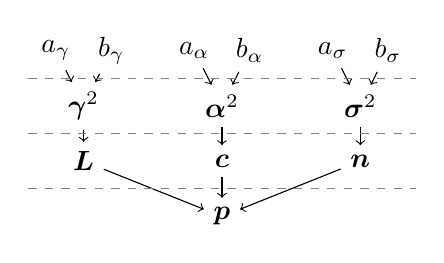
\begin{tikzpicture}
			\node(a1) at (0,0) {$a_{\gamma}$};
			\node(b1) at ($(a1)+(2em,0)$) {$b_{\gamma}$};
			\node(a2) at ($(b1)+(3em,0)$) {$a_{\alpha}$};
			\node(b2) at ($(a2)+(2em,0)$) {$b_{\alpha}$};
			\node(a3) at ($(b2)+(3em,0)$) {$a_{\sigma}$};
			\node(b3) at ($(a3)+(2em,0)$) {$b_{\sigma}$};
			
			\node at ($(a1)!0.5!(b1)+(0,-2em)$) (gam) {$\bm{\gamma}^2$};
			\node at ($(a2)!0.5!(b2)+(0,-2em)$) (alp) {$\bm{\alpha}^2$};
			\node at ($(a3)!0.5!(b3)+(0,-2em)$) (sig) {$\bm{\sigma}^2$};
			
			\draw[->] (a1)--(gam);
			\draw[->] (b1)--(gam);
			\draw[->] (a2)--(alp);
			\draw[->] (b2)--(alp);
			\draw[->] (a3)--(sig);
			\draw[->] (b3)--(sig);
			
			\node at ($(gam)+(0,-2em)$) (L) {$\bm{L}$};
			\node at ($(alp)+(0,-2em)$) (c) {$\bm{c}$};
			\node at ($(sig)+(0,-2em)$) (n) {$\bm{n}$};
			
			\draw[->] (gam)--(L);
			\draw[->] (alp)--(c);
			\draw[->] (sig)--(n);
			
			\node at ($(c)+(0,-2em)$) (p) {$\bm{p}$};
			
			\draw[->] (L)--(p);
			\draw[->] (c)--(p);
			\draw[->] (n)--(p);
			
			%hline
			\draw[dashed,color=gray]  ($(a1)+(-1em,-1em)$) -- ($(b3)+(1em,-1em)$) ;
			\draw[dashed,color=gray]  ($(a1)+(-1em,-3em)$) -- ($(b3)+(1em,-3em)$) ;
			\draw[dashed,color=gray]  ($(a1)+(-1em,-5em)$) -- ($(b3)+(1em,-5em)$) ;		
		\end{tikzpicture}
	\end{minipage}
	\vfill
	\begin{minipage}{\textwidth}
			Gibbs sampling: update successively each variable			
			\begin{center}				
				\begin{minipage}{0.9\textwidth}
					\begin{algorithmic}
						\REQUIRE $\bm{p},~a_\gamma^{(0)},~b_\gamma^{(0)},~a_\alpha^{(0)},~b_\alpha^{(0)},~a_\sigma^{(0)},~b_\sigma^{(0)}$ % \hfill\parbox{6cm}{$\triangleright$ \textit{computes eigenvalues}}\\
						\FOR{$k$}
							\STATE~~~~ sample $\bm{c}$ in $[\bm{c}~|~\bm{p},\bm{L}^{(k-1)},\bm{\gamma}^{(k-1)},\bm{\alpha}^{(k-1)},\bm{\sigma}^{(k-1)} ]$\\
							\STATE~~~~ sample $\bm{L}$ in $[\bm{L}~|~\text{rest}  ]$\\
							\STATE~~~~ sample $\bm{\gamma}^2$ in $[\bm{\gamma}^2~|~ \text{rest}  ]$\\
							\STATE~~~~ sample $\bm{\alpha}^2$ in $[\bm{\alpha}^2~|~\text{rest}  ]$\\
							\STATE~~~~ sample $\bm{\sigma}^2$ in $[\bm{\sigma}^2~|~ \text{rest}  ]$\\
						\ENDFOR
					\end{algorithmic}
				\end{minipage}				
			\end{center}
	\end{minipage}
\end{frame}

\setcounter{framenumber}{\value{finalframe}}




%Texte du diapo \cite{Solomaa1973} et \cite{Dijkstra1982}
%\vfill
% 
%{\tiny 
%\usebibitemtemplate{\color{black}\insertbiblabel} 
%\usebibliographyblocktemplate{\color{black}}{\color{black}}{\color{black}}{\color{black}} 
% 
%\begin{thebibliography}{} 
%\bibitem{Solomaa1973} 
%A.~Salomaa. 
%\newblock {\em Formal Languages}. 
%\newblock Academic Press, 1973. 
%\bibitem{Dijkstra1982} 
%E.~Dijkstra. 
%\newblock Smoothsort, an alternative for sorting in situ. 
%\newblock {\em Science of Computer Programming}, 1(3):223--233, 1982. 
%\end{thebibliography} }


\end{document}